\documentclass[acmtog,nonacm]{acmart}
\settopmatter{printacmref=false,printccs=true,printfolios=true}
\setcopyright{none}
\renewcommand\footnotetextcopyrightpermission[1]{}
\pagestyle{plain}
\usepackage{booktabs,tikz,subcaption}
\usetikzlibrary{positioning,arrows.meta}
\graphicspath{{figures/}}
\citestyle{acmauthoryear}
\newcommand{\bx}{\mathbf{x}}
\newcommand{\bu}{\mathbf{u}}
\newcommand{\bL}{\mathbf{L}}
\newcommand{\bS}{\boldsymbol{\Sigma}}
\newcommand{\sigz}{\sigma_0}
\newcommand{\sel}[1]{\emph{#1}}

\begin{document}
\title{Vortex Gaussians: Simulation-Driven Fire and Smoke as Native Gaussian-Splatting Content}
\author{Zijun Xiao}
\affiliation{\institution{Georgia Institute of Technology}\city{Atlanta}\state{Georgia}\country{USA}}
\email{zxiao316@gatech.edu}

\begin{abstract}
A vortex particle and a 3D Gaussian are the same object seen from two disciplines. We build a fire and smoke system on that identity: the splats a rasterizer draws are the elements a vortex method integrates, so velocity, its analytic gradient and temperature are closed-form functionals of the population already on screen, with no grid and no linear solve. The identity has a consequence no volume-based compositor can reproduce: flame and reconstruction share one depth-sorted emission--absorption pass, so fire transmits partially through a semi-transparent foreground. On a benchmark capture with foliage in front of the flame, 88.1\% of the silhouette is partially transmitted under our composition against 9.1\% for the strongest per-pixel depth-tested baseline at matched fire energy; on an opaque occluder the two tie. Combustion state lives on the scene's own Gaussians, so the flame ignites the reconstruction and burning geometry re-seeds the solver.

The fire alone runs at 58\,FPS on a desktop GPU and 22\,FPS on an integrated one (5.4k Gaussians, $1280\times800$, single-threaded CPU JavaScript simulation). Composited with a 729\,826-Gaussian reconstruction it runs at 3.4\,FPS, and the combustion loop on a capture is six to eleven times slower than real time. We report each approximation against what it replaces: the treecode against the exact sum, the grid-free solver against vortex-in-cell, and the layered decomposition against a true 3D vortex-particle solver.
\end{abstract}

\begin{CCSXML}
<ccs2012><concept><concept_id>10010147.10010371.10010352.10010379</concept_id><concept_desc>Computing methodologies~Physical simulation</concept_desc><concept_significance>500</concept_significance></concept><concept><concept_id>10010147.10010371.10010372.10010373</concept_id><concept_desc>Computing methodologies~Rasterization</concept_desc><concept_significance>300</concept_significance></concept></ccs2012>
\end{CCSXML}
\ccsdesc[500]{Computing methodologies~Physical simulation}
\ccsdesc[300]{Computing methodologies~Rasterization}
\keywords{Gaussian splatting, fire, smoke, vortex particle methods, Barnes--Hut treecode, emissive media}

\begin{teaserfigure}
\centering
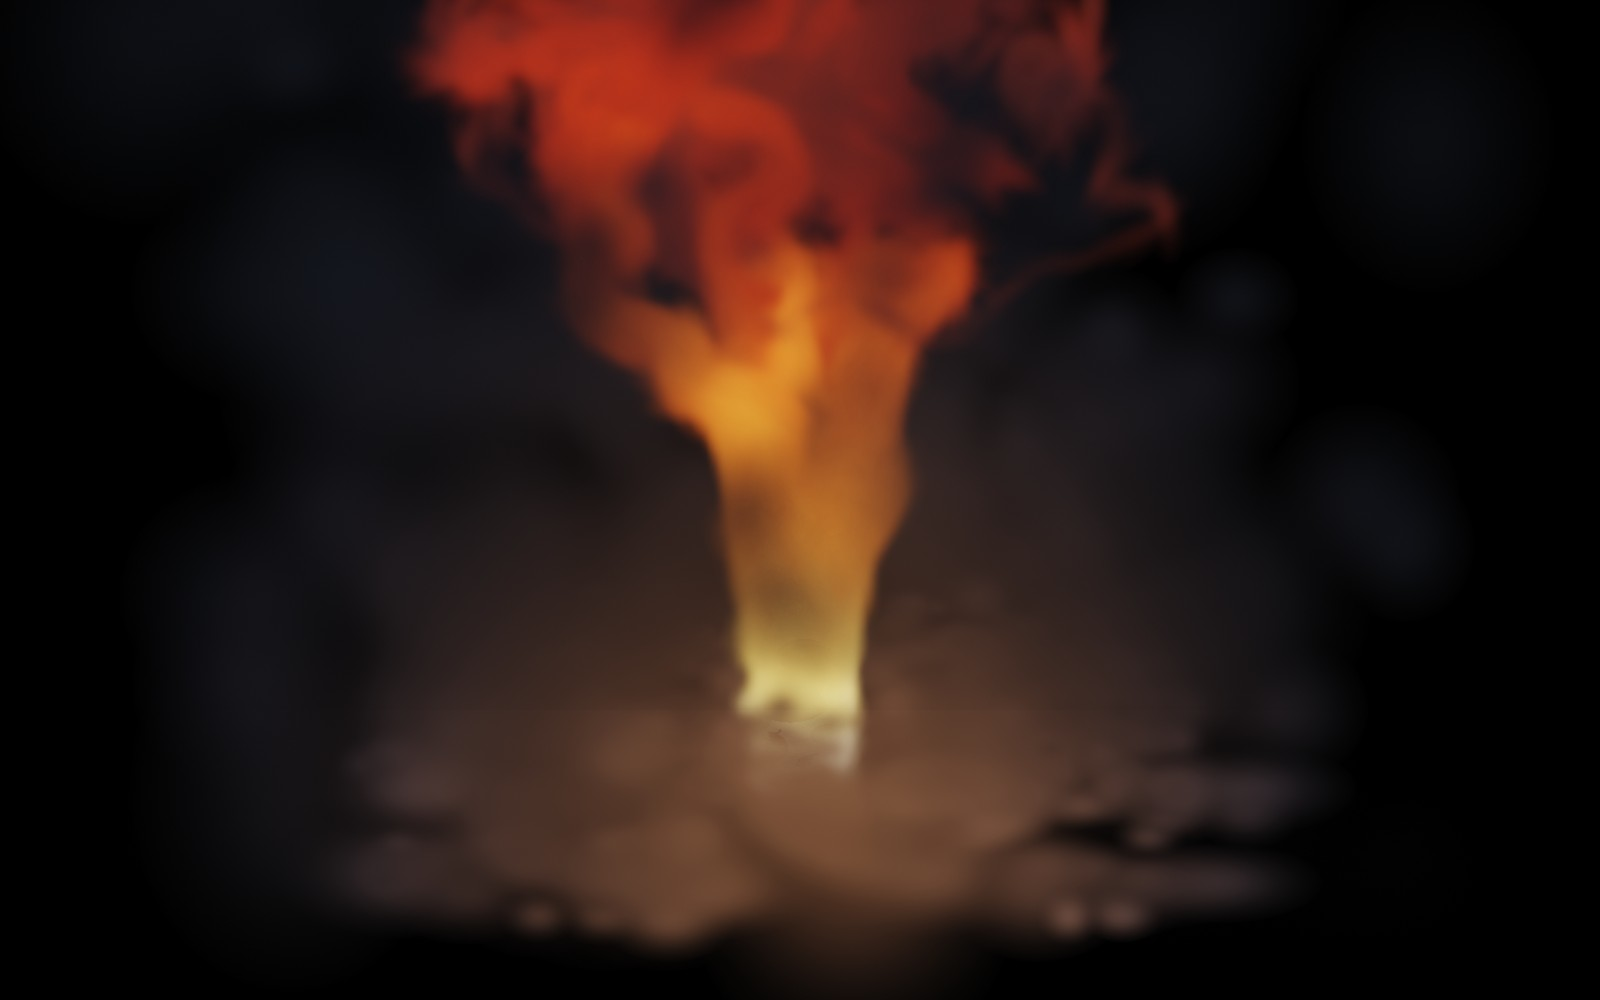
\includegraphics[height=3.72cm]{teaser_flame}\hfill
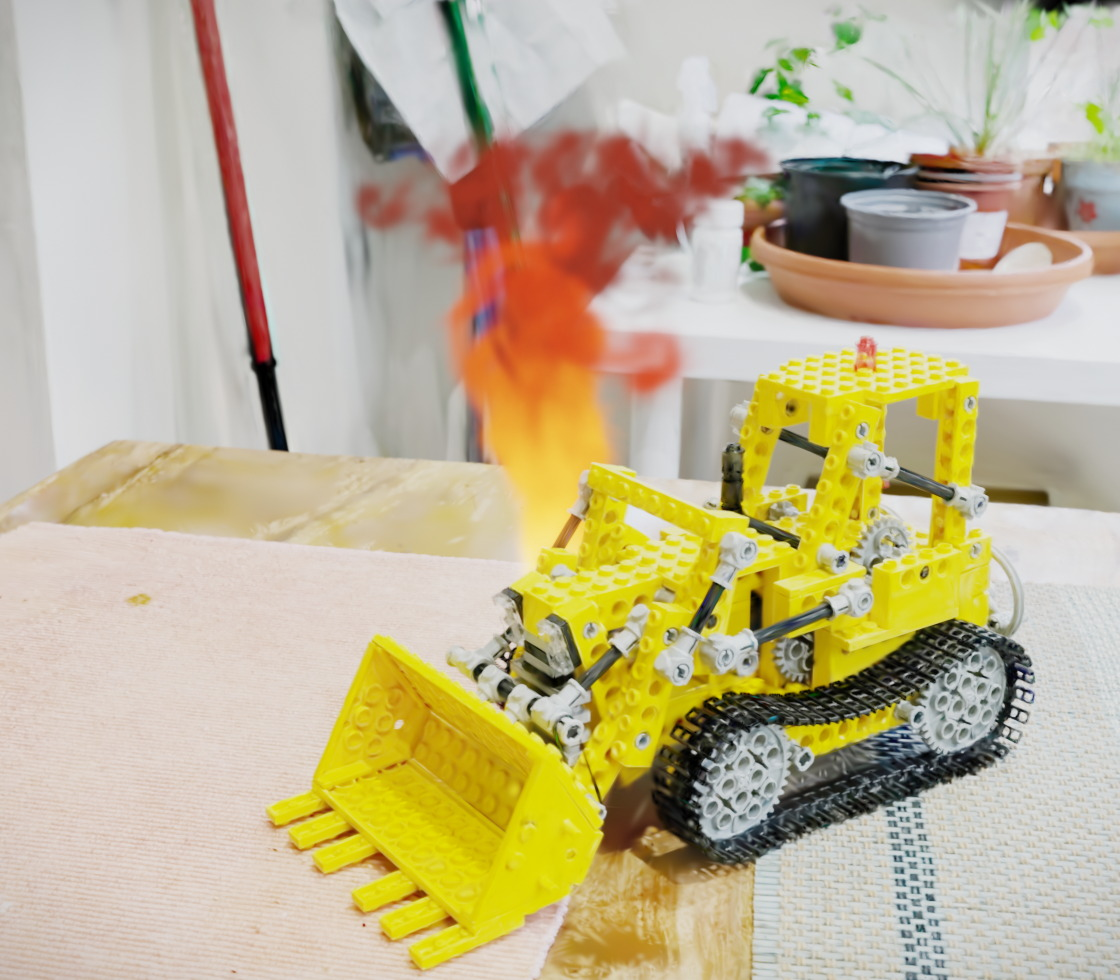
\includegraphics[height=3.72cm]{teaser_kitchen}\hfill
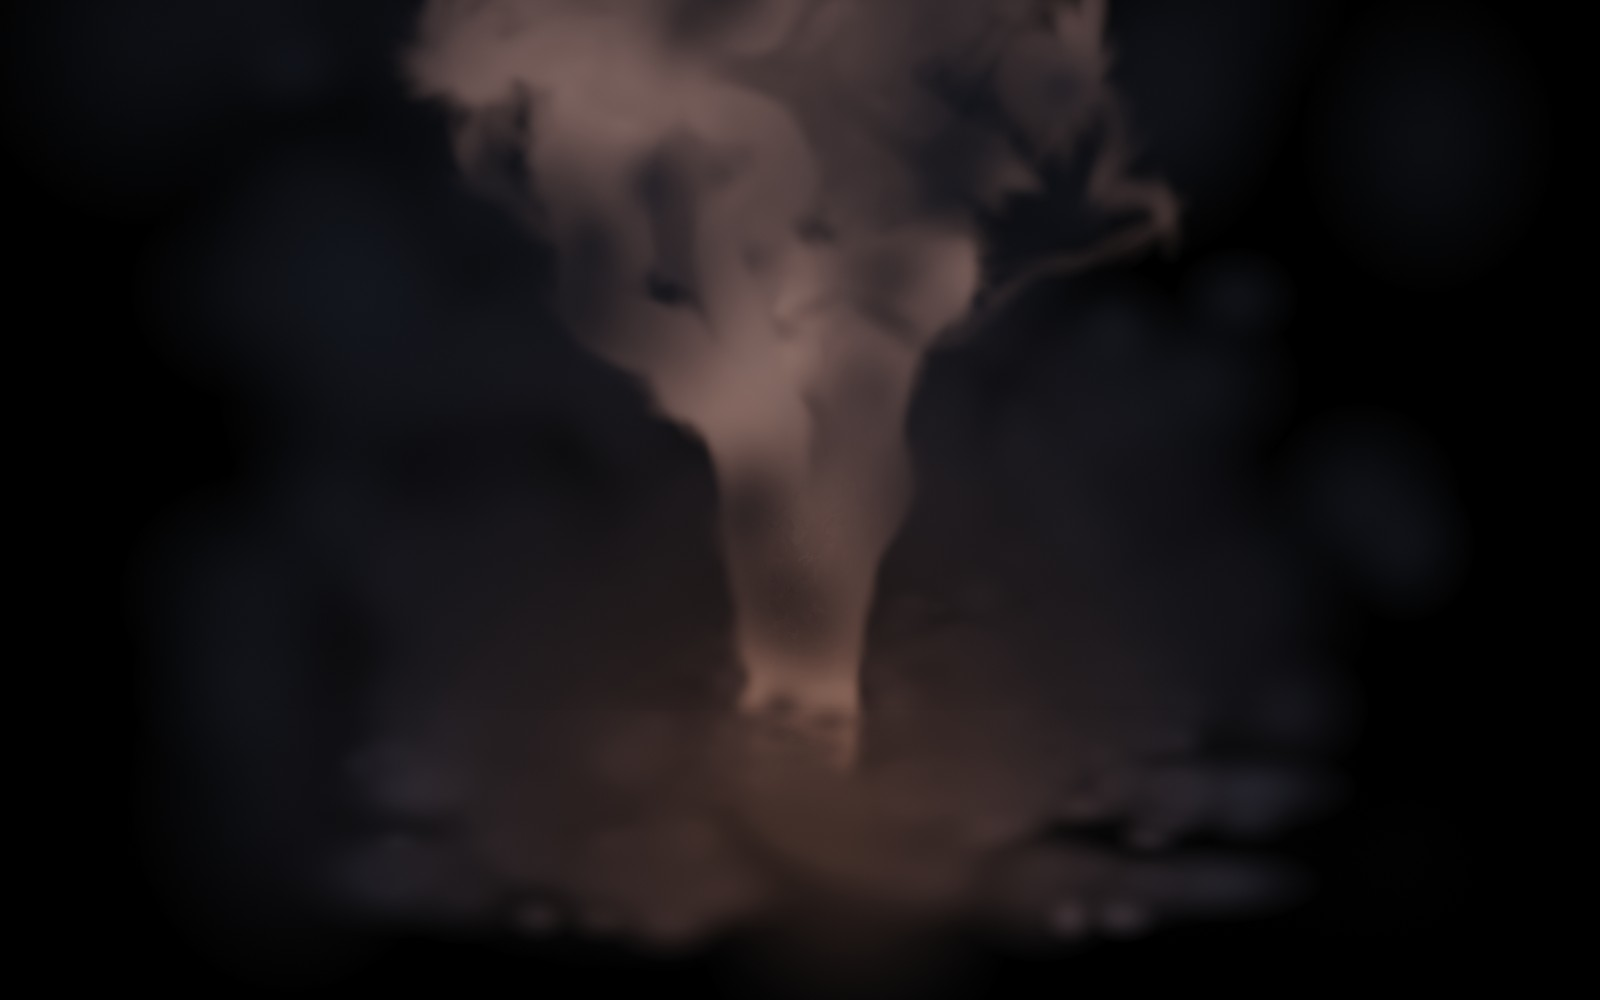
\includegraphics[height=3.72cm]{teaser_smoke}
\caption{Fire and smoke as Gaussian-splatting content. \emph{Left:} nine layered 2D grid-free vortex-particle simulations in which every vortex element is an emissive anisotropic Gaussian; this fire runs at 58\,FPS. \emph{Middle:} the same solver inside \emph{kitchen} from Mip-NeRF 360 \cite{barron2022,kerbl2023} (729\,826 Gaussians); flame and scene share one depth order, so the loader's arms occlude the fire per primitive. The scene adds 272\,ms of rasterization, for 3.4\,FPS. \emph{Right:} the identical particle set re-shaded as smoke.}
\label{fig:teaser}
\end{teaserfigure}

\maketitle

\section{Introduction}
Gaussian splatting made captured environments renderable in real time \cite{kerbl2023}, and physics-integrated methods now animate them: elastic solids and liquids follow continuum solvers attached to the reconstructed primitives \cite{xie2024,feng2025,jiang2024,zhong2024}. Fire and smoke are missing from this picture. Existing Gaussian flames are inverse: they reconstruct an observed fire and can only replay it \cite{shui2024,nazarenus2025}. The one system that synthesizes new fire in reconstructed scenes, FieryGS \cite{shen2026}, runs an offline $256^3$ Eulerian solver and ray-marches the result over the scene, treated as an opaque backdrop, at seconds per frame.

That composition is the limit this paper addresses. A volume rendered separately from a reconstruction can be depth-tested against it, but a depth buffer holds one surface per pixel, and a reconstruction's foliage, hair and soft edges are not one surface. They are many low-opacity primitives with air between them. A flame behind them should be partly seen through each, and no depth test can express that.

Our starting point is that a Lagrangian vortex particle and a 3D Gaussian are the same kind of object: unordered point primitives with a position and a few attributes, consumed by a sort-and-blend operator. We take this literally. One particle set is simultaneously the simulation state and the render primitive. The rasterizer reads each vortex particle as an emissive anisotropic Gaussian whose mean is the particle position, whose colour follows temperature, and whose covariance is transported by the local velocity gradient.

This identity is valuable because of what it makes possible, rather than because it removes a conversion step. Since fire and scene are one population, three things follow that a backdrop or depth-tested volume cannot provide:
\begin{itemize}
\item \textbf{Partial transmittance through a captured scene.} Flame and scene primitives interleave in one sorted pass, so a flame behind foliage receives a continuous transmittance. We measure 88.1\% of a flame's silhouette partially transmitted against 9.1\% for the strongest depth-tested baseline, when that baseline is handed the threshold matching our fire energy (\S\ref{sec:occlusion}).
\item \textbf{Combustion on the scene's own primitives.} Heat, fuel and char are per-splat attributes of the reconstruction. Burning writes into the same primitives the renderer draws, and burning splats feed particles back into the solver (\S\ref{sec:loop}).
\item \textbf{Scene coupling at particle cost.} Because the flame is a particle set in world space, it can light the scene as a few clustered point sources and feel it through closed-form boundary terms, with no volume in between (\S\ref{sec:light}, \S\ref{sec:deflect}).
\end{itemize}
Our contributions are:
\begin{itemize}
\item \textbf{An identity between simulation degrees of freedom and rendered primitives for a gas.} Each splat carries a Lamb--Oseen vortex core at its own mean, and velocity, its gradient and temperature are closed-form functionals of that population. The gradient transports the rendered covariance, so splat shape is a solver output. Gases have no rest configuration, and vorticity-carrying particles supply the rest-configuration-free counterpart of covariance-from-deformation for solids \cite{xie2024}.
\item \textbf{A closed combustion and composition loop between a forward flame and the splats of a captured scene.} On a public benchmark the flame ignites a table strip, the front crosses to the object resting on it, and that object ignites at $t=24.40$\,s with nothing lit by hand. The spread physics is conventional \cite{pirk2017,hadrich2021}; the substrate and the closed loop are what is new.
\end{itemize}
The dynamics that make this affordable are a grid-free instance of the layered architecture of production fire \cite{horvath2009}: stacked 2D Gaussian vortex-particle slices under a Barnes--Hut treecode. Gaussian blobs, treecodes and SPH estimation are classical, and we claim an engineering synthesis here rather than a fluids advance. Its one distinctive property is that the accelerator, the director field and the picture are all Gaussians. Because every field is closed-form, every approximation can be measured against the thing it replaces (\S\ref{sec:eval}).

\section{Related Work}
\paragraph{Fire and smoke simulation.} Gaseous simulation in graphics descends from stable semi-Lagrangian advection \cite{stam1999} and vorticity confinement \cite{fedkiw2001,steinhoff1994}, specialized to combustion by \citet{nguyen2002}. Heat-threshold spread with fuel and charring is established on botanical meshes \cite{pirk2017} and at wildfire scale \cite{hadrich2021}. Vortex methods discretize the vorticity form of the Euler equations on Lagrangian elements \cite{chorin1973,cottet2000,park2005,selle2005}, filaments \cite{angelidis2005,weimann2010} or sheets \cite{brochu2012,pfaff2012}. Their bottleneck is velocity recovery, addressed by particle--grid hybrids, which reintroduce a grid, or by treecodes and fast multipole methods \cite{barnes1986,greengard1987,lindsay2001}. \citet{zhang2014} brought fast summation to graphics with a far field on a mesh; ours is itself a set of Gaussians. Vortex-particle flow maps \cite{wang2025} are high-accuracy and offline where we trade accuracy for a real-time rendering loop. Our Gaussian elements are classical \cite{beale1985,leonard1980}; the Lamb--Oseen core is chosen because its velocity and gradient are closed-form and because its profile is literally the rendered footprint.

\paragraph{Production layered fire.} \citet{horvath2009} decompose film fire into a coarse directable pass and independent camera-facing 2D slices, offline at $\sim\!20$\,s per slice per frame on a GPU farm, at resolutions orders of magnitude above ours. We replace per-slice grid Navier--Stokes with grid-free vortex particles, slice textures with Gaussians shared with the environment, and the fixed projection kernel with a tunable coarse field. We do not claim to make that system real-time; we build an interactive-scale instance of its architecture.

\paragraph{Gaussian splatting.} 3DGS \cite{kerbl2023} follows the EWA splatting lineage \cite{zwicker2001}. \citet{condor2025} show Gaussian mixtures are a sound basis for emissive media under ray tracing; we target the rasterized end of that trade-off. Dynamic extensions obtain motion from data \cite{luiten2024,wu2024} and replay it. Physics-integrated Gaussians animate scenes forward \cite{xie2024,feng2025,zhong2024,jiang2024}, but all target media with material points or surfaces. Closest in spirit, Gaussian Fluids \cite{xing2025} also solves fluids on Gaussian degrees of freedom, by the opposite mechanism: basis functions of a weak-form velocity field, advanced by optimization at 38--228\,s per step and visualized by separate passes. We treat Gaussians as explicit strong-form vortex elements that are themselves the picture.

\paragraph{Gaussians for fire.} FlameGS \cite{shui2024} and Gaussians on Fire \cite{nazarenus2025} reconstruct flames; PINF \cite{chu2022}, HyFluid \cite{yu2023} and FluidNexus \cite{gao2025} recover smoke or fluid from video. FieryGS \cite{shen2026} is the closest prior system. It infers material properties we do not, and shades Gaussians with a diffuse and specular term from voxels above a temperature threshold, at 2.37\,s per frame. Table~\ref{tab:position} summarizes the differences.

\begin{table}
\caption{Positioning. GS-native means rendered as Gaussian primitives depth-interleaved with the scene. Real time refers to the phenomenon alone; \S\ref{sec:cost} gives the composited cost.}
\label{tab:position}
\footnotesize
\setlength{\tabcolsep}{3pt}
\begin{tabular}{lcccccc}
\toprule
& gaseous & forward & real & GS- & grid-free & scene \\
& emissive & physics & time & native & solver & composed \\
\midrule
\citet{horvath2009} & \checkmark & \checkmark & --- & --- & --- & matte \\
PhysGaussian & --- & \checkmark & --- & \checkmark & --- & \checkmark \\
Gaussian Splashing & --- & \checkmark & --- & \checkmark & \checkmark & \checkmark \\
Gaussian Fluids & --- & \checkmark & --- & --- & \checkmark & --- \\
Fire reconstruction & \checkmark & --- & (render) & \checkmark & n/a & --- \\
VR-GS & --- & \checkmark & \checkmark & \checkmark & --- & \checkmark \\
FieryGS & \checkmark & \checkmark & --- & --- & --- & backdrop \\
Ours & \checkmark & \checkmark & \checkmark & \checkmark & \checkmark & \checkmark \\
\bottomrule
\end{tabular}
\end{table}

\section{Overview}
The domain is a stack of $N$ parallel slice layers (default $N=9$). Once per frame we rebuild each layer's Barnes--Hut tree, merge its top levels into a coarse director field, and advance each layer's 2D Gaussian vortex-particle simulation. The renderer lifts each particle into world space and instances one emissive Gaussian per particle. Any layer can be swapped at runtime between the solver and a procedural curl-noise plume \cite{bridson2007}, which serves as an ablation instrument.

The identity has precise edges. The 2.5D decomposition is a modelling choice, priced in \S\ref{sec:layered}. Tree, Morton sort and spatial hash are index structures rebuilt from particles, not field state. Velocity induction uses each particle's isotropic core $\sigma_i$; the rendered covariance is that core's flow-sheared envelope, sharing mean and scale but not orientation. Particles carry a dynamics temperature and a colour temperature, two scalar fields over the same means and kernels. Circulation is solver state that reaches the screen only through the motion it induces. The vortex core $\sigz$ is a regularization length, while on-screen splat size is a display scale coupled to it only through the overlap condition (\S\ref{sec:treecode}). The defensible claim is one population, one set of means, every solver field a closed-form functional of it, and no intermediate field representation.

\section{Layered Gaussian Vortex Simulation}
\subsection{Per-slice dynamics}
Each slice simulates buoyant flow in vorticity form. In 2D the stretching term vanishes, leaving
\begin{equation}
\frac{\partial\omega}{\partial t}+(\bu\cdot\nabla)\omega=\beta\,\frac{\partial T}{\partial x},
\label{eq:vort}
\end{equation}
where the baroclinic source injects the counter-rotating pairs that roll rising columns into mushroom caps \cite{nguyen2002,selle2005}. Each particle $i$ is a Gaussian vortex element with circulation $\Gamma_i$ and core $\sigma_i$, so the vorticity field is the rendered mixture
\begin{equation}
\omega(\bx)=\sum_j\Gamma_j\,G_{\sigma_j}(\bx-\bx_j),\qquad G_\sigma(\mathbf r)=\frac{1}{2\pi\sigma^2}e^{-\|\mathbf r\|^2/2\sigma^2}.
\label{eq:mixture}
\end{equation}
Each frame performs four grid-free steps.

\emph{Temperature.} Particles carry a dynamics temperature $T_i$, heated in the source band and cooled linearly. Advection is free because the carrier advects. The field is the Shepard-normalized mixture
\begin{equation}
\tilde T(\bx)=\frac{\sum_j T_j w_j(\bx)}{\sum_j w_j(\bx)},\qquad w_j(\bx)=e^{-\|\bx-\bx_j\|^2/4\bar\sigma_j^2}.
\end{equation}

\emph{Baroclinic injection.} Each particle accumulates circulation from the moment-renormalized gradient of that mixture \cite{monaghan1992}, which is exact for linear fields under any particle distribution:
\begin{equation}
\Gamma_i\leftarrow(1-\lambda_\Gamma\Delta t)\Gamma_i+\Delta t\,\beta\,
\frac{\sum_j(T_j-T_i)(x_j-x_i)w_{ij}}{\sum_j(x_j-x_i)^2w_{ij}}.
\label{eq:baro}
\end{equation}

\emph{Velocity and gradient.} The mixture induces the Lamb--Oseen velocity \cite{lamb1932,saffman1992}
\begin{equation}
\bu(\bx)=\sum_j\frac{\Gamma_j}{2\pi}\frac{(-r_y,r_x)}{\|\mathbf r_j\|^2}\left(1-e^{-\|\mathbf r_j\|^2/2\sigma_j^2}\right),\quad\mathbf r_j=\bx-\bx_j.
\label{eq:lo}
\end{equation}
It is regular at the origin, solenoidal term by term, and reduces to the point-vortex kernel beyond a few $\sigma$. Its gradient $\bL=\nabla\bu$ is closed-form and accumulated in the same sum at marginal cost.

\emph{Advection.} Each particle adds direct buoyancy $\beta_b\tilde T(\bx_i)\hat{\mathbf y}$, a small curl-noise perturbation, wind and the director nudge, then advects with explicit Euler. Direct buoyancy is a control force with its own gain, and $\nabla\cdot(\beta_bT\hat{\mathbf y})\neq0$ in a plume. The solver therefore needs no linear solve, but the advecting velocity is not divergence-free; only the recovered field of Eq.~\ref{eq:lo} is.

Particles also carry a colour temperature cooled as $\mathrm dT^c_i/\mathrm dt=-\kappa(T^c_i)^2$, which concentrates brightness at the hot base. Particles are recycled when cold, exhausted or out of bounds, so the Gaussian count stays bounded.

\subsection{Treecode and director field}
\label{sec:treecode-method}
We accelerate Eq.~\ref{eq:lo} with a Barnes--Hut quadtree \cite{barnes1986} rebuilt each frame. Each node aggregates its subtree into a moment-matched super-Gaussian: signed circulation, an $|\Gamma|$-weighted centroid, a signed dipole moment that restores the effect of sign cancellation, and a matched core $\sigma_c^2=\sum_j|\Gamma_j|(\sigma_j^2+\|\bx_j-\bx_c\|^2)/\sum_j|\Gamma_j|$. A far node is itself a Gaussian vortex element, evaluated by Eq.~\ref{eq:lo}.

Independent slices produce $N$ uncorrelated fires. The top levels of the per-layer trees, merged across slices into at most 16 super-Gaussians plus their images through the ground plane with negated circulation, define a global velocity field $\mathbf U$. The images restore a no-penetration floor without a boundary grid. Every particle is nudged toward it:
\begin{equation}
\bu_i\leftarrow\bu_i+c\,(\mathbf U(\bx_i)-\bu_i),\qquad c\in[0,1].
\label{eq:couple}
\end{equation}
This is the two-level decomposition of \citet{horvath2009} with a continuously tunable coupling, and with both levels made of Gaussians.

Equation~\ref{eq:couple} couples every slice to a shared field but not to its neighbours. Particle pairs in adjacent slices can additionally exchange circulation through a symmetric weight,
\begin{equation}
\Gamma_i\mathrel{+}=\delta_{ij},\quad\Gamma_j\mathrel{-}=\delta_{ij},\quad\delta_{ij}=\Delta t\,\kappa_z\,\eta_{ij}(\Gamma_j-\Gamma_i),
\label{eq:pse}
\end{equation}
a particle-strength-exchange discretization \cite{degond1989} of the out-of-plane transport the stacking deletes. Total circulation is conserved exactly by antisymmetry. It models the dropped coupling, not true 3D stretching, and it is a diffusion: \S\ref{sec:layered} measures both its gain and its price. It is off in the shipping look.

\subsection{Slice geometry}
Layer $k$ sits at depth offset $z_k=(k/(N-1)-\tfrac12)D$. In the default view-aligned mode the in-plane axes are the camera's horizontal right vector and world up. Because solver state lives on particles, re-orienting the stack changes only the lift of in-plane coordinates into world space, at no re-simulation cost. A world-fixed mode pins slices to a world plane; seen edge-on those slices lose up to 89\% of their radiant energy, while view-aligned slices are azimuth-invariant to numerical precision.

\section{Emissive Gaussian Rendering}
\begin{figure*}
\centering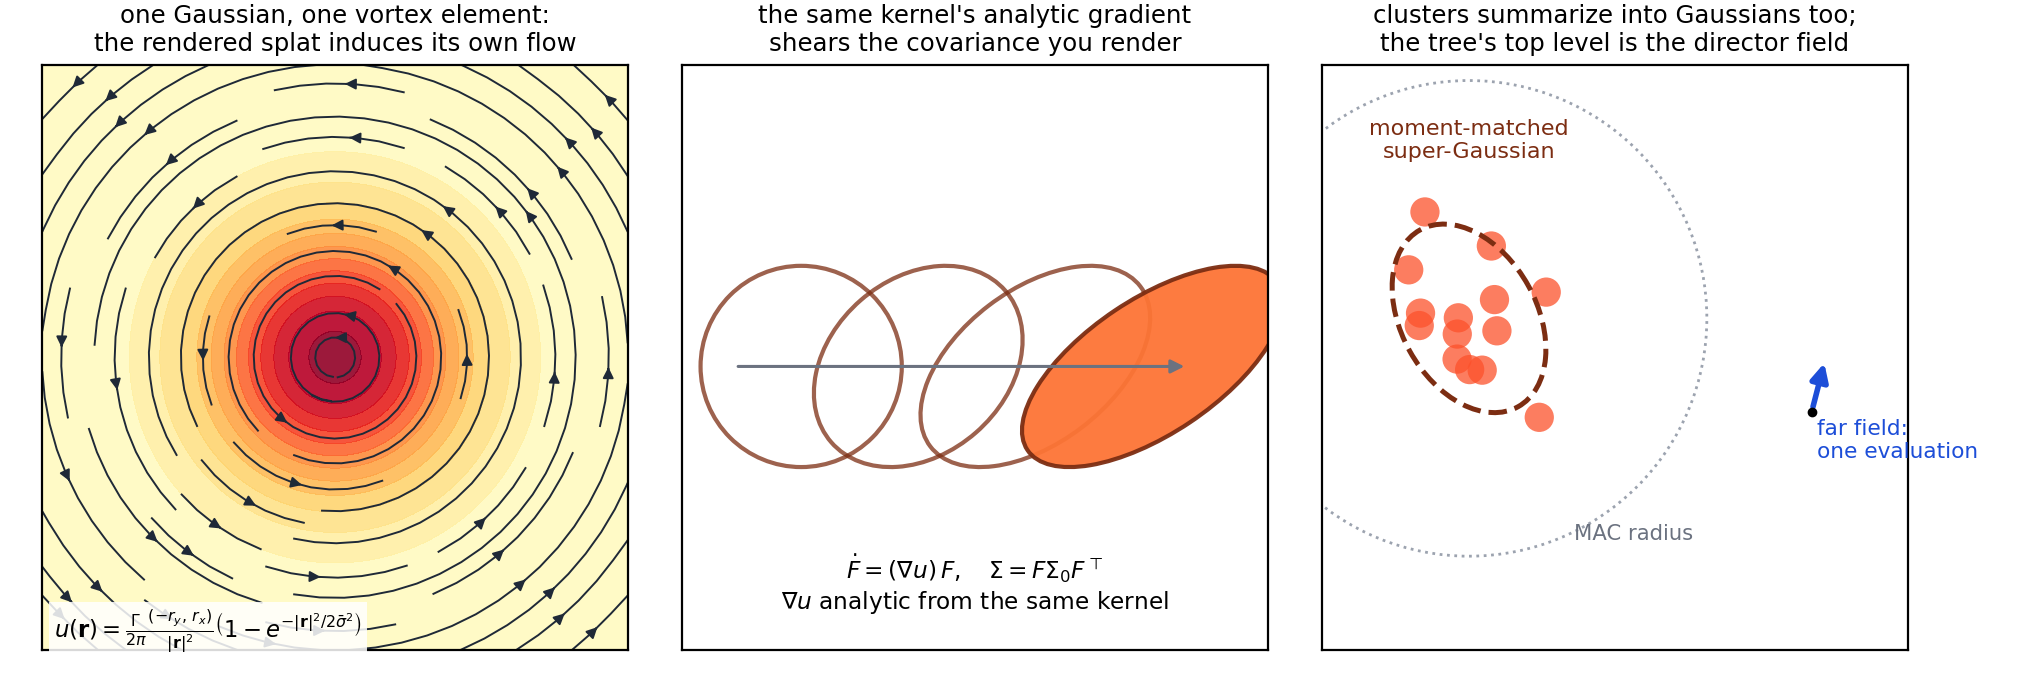
\includegraphics[width=0.86\textwidth]{identity}
\caption{One Gaussian, three closed-form roles. \emph{Left:} the rendered splat is a Lamb--Oseen vortex element. \emph{Middle:} the kernel's analytic gradient drives the rendered covariance. \emph{Right:} tree clusters are moment-matched super-Gaussians, and the top level doubles as the director field.}
\label{fig:identity}
\end{figure*}

\paragraph{Mapping.} Each attribute of the rendered Gaussian is read directly off the particle: mean from position by slice lift, colour from temperature by a blackbody ramp \cite{nguyen2002,pegoraro2006}, opacity from density, and covariance from the velocity gradient (Figure~\ref{fig:identity}).

\paragraph{Flow-driven covariance.} Isotropic splats read as bubbles; flames are sheared into streaks. We evolve each particle's in-plane covariance by the analytic gradient,
\begin{equation}
\dot\bS=\bL\bS+\bS\bL^\top,
\label{eq:cov}
\end{equation}
relaxed toward identity and stabilized in closed form by renormalizing $\det\bS=1$ and clamping the leading eigenvalue, which bounds the axis ratio. Equation~\ref{eq:cov} is the differential form of PhysGaussian's $\bS=\mathbf F\bS_0\mathbf F^\top$ \cite{xie2024}; for a gas $\mathbf F$ is ill-defined without a rest configuration, so the incremental form is the natural one. Because the clamp acts on the rendered quantity, the sliver failure mode of Gaussians under sustained shear cannot occur.

\paragraph{Unified compositing.} All Gaussians are sorted front-to-back and rasterized into an RGBA16F target. Fragments output premultiplied $(c_i\alpha_i,\alpha_i)$ and blend as
\begin{equation}
C\leftarrow C+(1-A)c_i\alpha_i,\qquad A\leftarrow A+(1-A)\alpha_i,
\label{eq:blend}
\end{equation}
exactly the emission--absorption forward pass of 3DGS \cite{kerbl2023,zwicker2001}. The opacity footprint is a pedestal-subtracted Gaussian that falls smoothly to zero on the quad's inscribed circle. Flame, smoke, ember and scene fragments evaluate the same footprint with different weights: fire is optically thin and emission-dominated, smoke absorption-dominated, and the same particle state spans the range under two scalar controls. Radiance passes through bloom, ACES tone mapping \cite{narkowicz2016} and gamma.

\paragraph{Merging a reconstruction.} A loaded \texttt{.ply} renders with the full EWA projection and spherical harmonics up to degree 3. Scene splats are counting-sorted each frame into $K=1536$ view-depth buckets in $O(n+K)$, and the renderer walks the buckets near to far, interleaving ranges of the exactly sorted dynamic stream with ranges of the scene stream under one blend state. The bucketing has a measured bound: over 60 instrumented runs the largest out-of-order depth stayed below one bucket width, and inverted cross-stream pairs fall as $1/K$ (exponents $-0.989$ to $-1.011$). At $K=1536$ the shipping path reproduces an order-exact merge to 49.2--65.1\,dB. On \emph{kitchen} the flame spans 62 buckets for 9 slices, about $7\times$ finer than the slice spacing. The supplemental gives the full measurement.

\section{Coupling to the Scene}
\subsection{Combustion on the scene's primitives}
\label{sec:loop}
Each scene splat carries heat $h$, fuel $f$, a burning or charred state and a glow amount. Adjacency is a spatial hash over the prepared splats, and per-frame work is restricted to the fire front. A reconstruction carries no material labels, so fuel is authored per scene by a geometric rule.

The dynamics close a loop. \emph{Ignition:} sampled hot flame particles deposit heat into nearby splats; heat decays, so ignition requires sustained heating. \emph{Spread:} burning splats heat unburnt neighbours with a buoyant upward bias, following standard heat-driven models \cite{pirk2017,hadrich2021}. \emph{Consumption:} fuel depletes while an HDR glow term is added and char drives the splat's albedo toward soot at unchanged opacity. \emph{Feedback:} burning splats spawn hot particles in the nearest slice, which enter the temperature mixture directly, so ignited geometry grows its own plumes through the full baroclinic loop. What ignites next is therefore decided by the simulated flow as well as by an adjacency graph.

Char is a deposit that replaces albedo, so we desaturate to luminance and then dim, $\mathrm{mix}(c,\mathrm{grey}(c),0.85)\cdot0.12$. A plain multiply, the operator closest prior work uses \cite{shen2026}, preserves chromaticity, and a dark saturated yellow reads as olive.

\subsection{Fire lights the scene}
\label{sec:light}
Flame particles already are world-space emitters, so we cluster them into six point lights: two columns relative to the source, three bands in height. A fixed binning keeps cluster identity stable across frames, so lights do not jump. Each particle contributes $e_i=d_iT_i^2(0.25+0.85T_i)$, the form of its own emission, and particles below the soot crossover contribute nothing. A cluster's intensity is normalized by the particle budget, its spatial variance softens the inverse-square falloff near the source, and its colour is the emission-weighted blackbody tint.

3DGS stores no normals, but surface-hugging splats are flat, so a splat's shortest principal axis is its surface normal up to sign. For splat $s$ with albedo $\rho_s$, shortest axis $\mathbf n_s$ and flatness $\phi_s=1-\sigma_{\min}/\sigma_{\mathrm{mid}}$, the added irradiance over clusters $c$ is
\begin{equation}
E_s=\sum_c\frac{I_c}{q_c}\,\mathrm{lerp}\!\left(\tfrac12,\ \frac{|\mathbf n_s\cdot\mathbf L_c|}{\sqrt{q_c}},\ \phi_s\right),\quad q_c=\|\mathbf L_c\|^2+s_c,
\label{eq:light}
\end{equation}
so near-spherical splats fall back to the isotropic mean of $|\cos|$. The rendered radiance becomes $\rho_s(\ell+E_s)$ for scene brightness $\ell$. The evaluation runs per splat in the vertex shader. It reads particles and writes nothing, so determinism is untouched. It is a diffuse term, the reconstruction's baked radiance stands in for albedo, and it casts no shadows: light passes through occluders.

\subsection{The scene deflects the flame}
\label{sec:deflect}
The ground mirror of \S\ref{sec:treecode-method} imposes a boundary with a closed-form image. We extend the same idea to captured geometry. Opaque splats near the fire are grouped by a spatial hash into at most 48 sphere proxies. Each slice cuts each sphere into a circle of centre $\mathbf c$ and radius $a$, widened by half a layer spacing so thin objects cannot pass between slices. For a particle at $\mathbf r=\bx-\mathbf c$, $\rho=\|\mathbf r\|$, the leading term of the circle theorem is the potential-flow doublet
\begin{equation}
\bu_d(\mathbf r)=-\frac{a^2}{\rho^2}\left[2(\mathbf U_a\cdot\hat{\mathbf r})\,\hat{\mathbf r}-\mathbf U_a\right],
\label{eq:doublet}
\end{equation}
where $\mathbf U_a$ is the mean velocity of particles on the upstream half-ring. It is divergence- and curl-free, cancels the normal flow at $\rho=a$, and doubles the tangential flow at the shoulders. A smooth window ends it by $\rho=4a$. The doublet only cancels locally uniform flow, so two further terms act in the wall layer $\rho<1.15a$: the residual inward normal velocity is projected out and positions are returned to the surface, and surface slip $u_t$ enters the particle's circulation at rate $\dot\Gamma=k\,u_t$, a surrogate for the boundary layer that gives the wake its roll-up.

No equation is solved and no grid is added. The pass costs $O(N_pm)$ for $m$ active circles. It runs on the 2D solver only, and it is off by default because it changes the simulation and hence the replay hash.

\section{Evaluation}
\label{sec:eval}
All measurements use a deterministic replay harness: every stochastic path draws from one seeded stream, the solver steps at fixed $\Delta t=1/60$\,s, and an FNV-1a hash over the full particle state fingerprints each frame. A run is determined by (seed, steps).

Two presets carry every number. \emph{Interactive} is $9\times600$ at $\theta=0.9$ ($\sim\!5.4$k flame Gaussians). \emph{Quality} is $9\times1300$ at $\theta=0.7$ ($\sim\!11.6$k). A third, \emph{Hero}, is an offline look for stills and video only (\S\ref{sec:hero}). Table~\ref{tab:params} lists the main parameters. World units are dimensionless unless a scene is calibrated against a real object.

\begin{table}
\caption{Key parameters. World domain $2\times3$ units.}
\label{tab:params}
\footnotesize
\begin{tabular}{llll}
\toprule
symbol & meaning & interactive / quality & eq. \\
\midrule
$N$ & slice layers & 9 / 9 & \\
$N_p$ & particles per layer & 600 / 1300 & \\
$\theta$ & treecode opening angle & 0.9 / 0.7 & \\
$\sigz$ & vortex core radius & 0.05 & \ref{eq:lo} \\
$\beta,\beta_b$ & baroclinic, direct buoyancy & 1.4, 0.9 & \ref{eq:baro} \\
$c$ & coarse coupling & 0.5 & \ref{eq:couple} \\
$\kappa_z$ & inter-slice exchange & 0 (optional) & \ref{eq:pse} \\
$D$ & stack depth & 0.7 & \\
$k_\Sigma,\kappa_{\max}$ & covariance gain, clamp & 1.3, 3.6 & \ref{eq:cov} \\
\bottomrule
\end{tabular}
\end{table}

\subsection{Cost}
\label{sec:cost}
Table~\ref{tab:cost} gives per-frame timings on the reference workstation, a Threadripper PRO 3945WX with an RTX 3080 under Chrome/ANGLE D3D11, as medians of five seeds with the simulation single-threaded in CPU JavaScript. Simulation cost per particle per frame is flat at 2.1--2.7\,$\mu$s across a $17\times$ span of element count.

\begin{table}
\caption{Fire-only cost per frame (ms) on the reference workstation at $1280\times800$. No scene is loaded. The first row group uses $\theta=0.7$; the last row is the shipping interactive preset at $\theta=0.9$. Grid baseline frame times and the full sweep are in the supplemental.}
\label{tab:cost}
\footnotesize
\setlength{\tabcolsep}{4pt}
\begin{tabular}{rrrrrrrr}
\toprule
$N$ & $N_p$ & Gauss. & sim VIC & sim VPM & sort & render & total (FPS) \\
\midrule
1 & 1300 & 1.3k & 1.32 & 3.1 & 0.40 & 0.58 & 4.1 (246) \\
5 & 1300 & 6.5k & 6.91 & 15.5 & 2.17 & 4.95 & 22.6 (44) \\
9 & 1300 & 11.6k & 12.9 & 29.8 & 4.24 & 7.77 & 41.8 (24) \\
17 & 1300 & 21.8k & 23.6 & 60.5 & 10.9 & 13.7 & 85.0 (12) \\
9 & 600 & 5.4k & 7.85 & 13.1 & 2.06 & 5.55 & 20.7 (48) \\
\midrule
9 & 600 & 5.4k & 7.85 & 10.4 & 1.74 & 5.05 & 17.1 (58) \\
\bottomrule
\end{tabular}
\end{table}

\paragraph{What real time covers.} The 58\,FPS figure is the fire alone. Rendering it inside a reconstruction is a separate draw cost, measured paired within one session at the interactive preset. The simulation step does not change. End to end the frame goes from 19.7\,ms (51\,FPS) to 36.4\,ms (28\,FPS) with the 45\,808-splat synthetic scene, 160.9\,ms (6.2\,FPS) with a 380k capture, and 292.4\,ms (3.4\,FPS) with the 729\,826-Gaussian \emph{kitchen}. The marginal cost per scene Gaussian is flat at $\sim\!0.37\,\mu$s (365, 375, 373\,ns), so the deficit is rasterization, independent of the solver. The fire is real-time, and the fire inside a multi-hundred-thousand-splat capture at this resolution is not.

\paragraph{Hardware.} Table~\ref{tab:hw} adds two further points from one machine, a Ryzen 9 9950X driving each of its two GPUs in turn under Chrome 156. Frames are synchronized with a pixel readback, and all rows are five-seed medians. Integrated graphics reaches 22\,FPS at the interactive preset. The simulation cost barely moves, since it runs on the CPU, and the deficit is entirely the draw. The integrated GPU here is a desktop Ryzen part, not a laptop; a thermally limited laptop would sit lower.

\begin{table}
\caption{Second and third hardware points, ms per frame at $1280\times800$, five-seed medians with GPU-synchronized timing. \emph{Scene} loads the 45\,808-splat synthetic capture with the world-space fire light on. \emph{Draw} includes gather and sort.}
\label{tab:hw}
\footnotesize
\begin{tabular}{llrrrr}
\toprule
GPU & configuration & sim & draw & total & FPS \\
\midrule
RTX 5070 Ti & interactive & 4.50 & 1.99 & 6.57 & 152 \\
 & quality & 12.03 & 4.76 & 16.51 & 61 \\
 & interactive + scene & 5.14 & 15.28 & 20.43 & 49 \\
 & quality + scene & 12.10 & 16.18 & 28.27 & 35 \\
\midrule
Radeon iGPU & interactive & 5.26 & 39.31 & 44.55 & 22 \\
 & quality & 9.96 & 88.00 & 97.78 & 10 \\
 & interactive + scene & 4.46 & 64.37 & 68.83 & 15 \\
 & quality + scene & 9.58 & 112.57 & 122.28 & 8 \\
\bottomrule
\end{tabular}
\end{table}

\subsection{Composition against semi-transparent occluders}
\label{sec:occlusion}
This is the central test of the composition claim. We compare against a ladder of baselines inside our own renderer, so the only variable is the compositing structure. The \emph{depth-aware} baseline is the strongest alternative we can build without interleaving: scene splats whose footprint opacity exceeds a threshold write depth, and fire fragments are $z$-tested against it. The \emph{backdrop} baseline composites the flame over the sorted scene, the structure of FieryGS \cite{shen2026}.

\begin{figure}
\centering
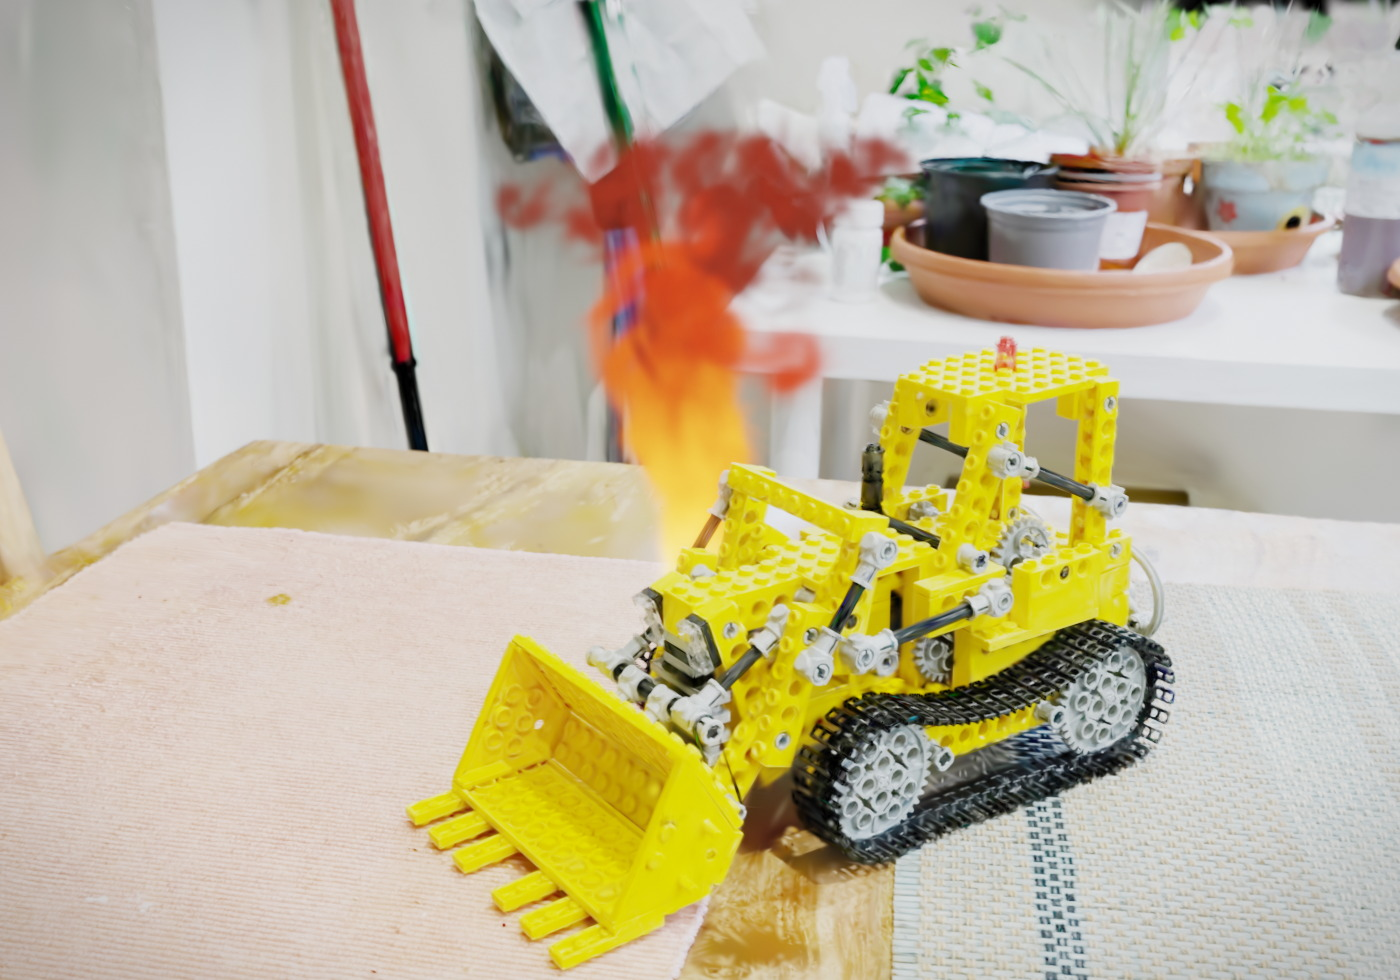
\includegraphics[width=.492\linewidth]{kitchen_ours}\hfill
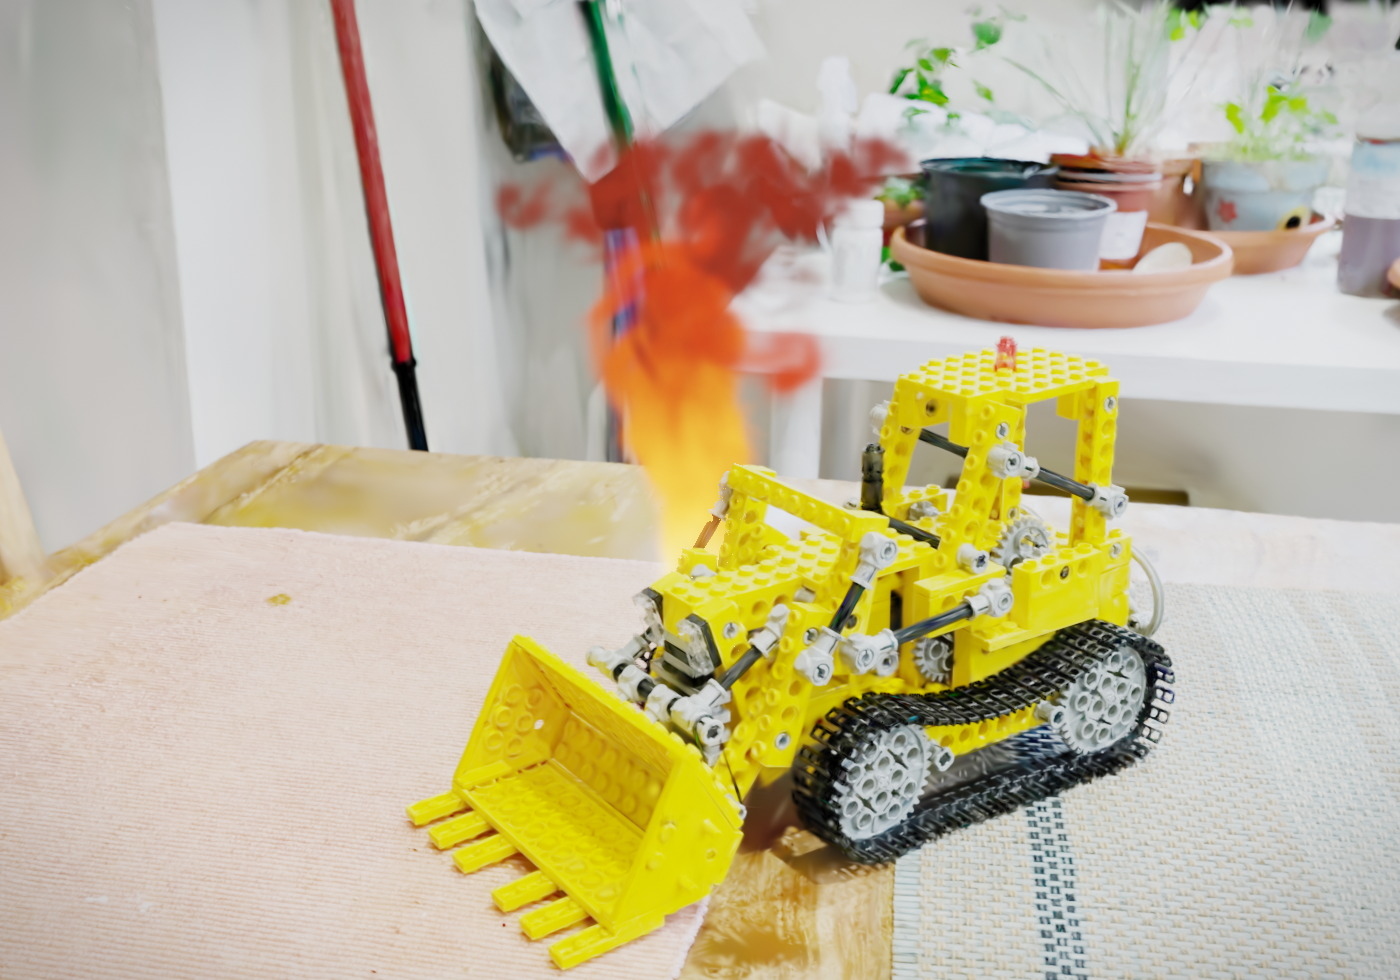
\includegraphics[width=.492\linewidth]{kitchen_depth}
\caption{An opaque occluder: \emph{kitchen}, with the fire behind the model loader. \emph{Left:} ours. \emph{Right:} depth-aware baseline, 100.4\% of our fire contribution. Over the flame's silhouette 85.5\% is fully transmitted, 12.0\% fully blocked and 2.5\% partial, and binary occlusion is what a $z$-test expresses. This tie is the control for Figure~\ref{fig:treehill}.}
\label{fig:kitchen}
\end{figure}

\paragraph{Opaque occluder.} On \emph{kitchen} the occluder is opaque plastic (Figure~\ref{fig:kitchen}). The depth-aware baseline ties with us, at 99.9--110.2\% of our fire contribution across thresholds 0.15--0.90, differing in 3\,134 of 1\,372\,000 pixels at 0.50. The backdrop baseline puts the white-hot base in front of the arms that should hide it (119.3\%).

\begin{figure*}
\centering
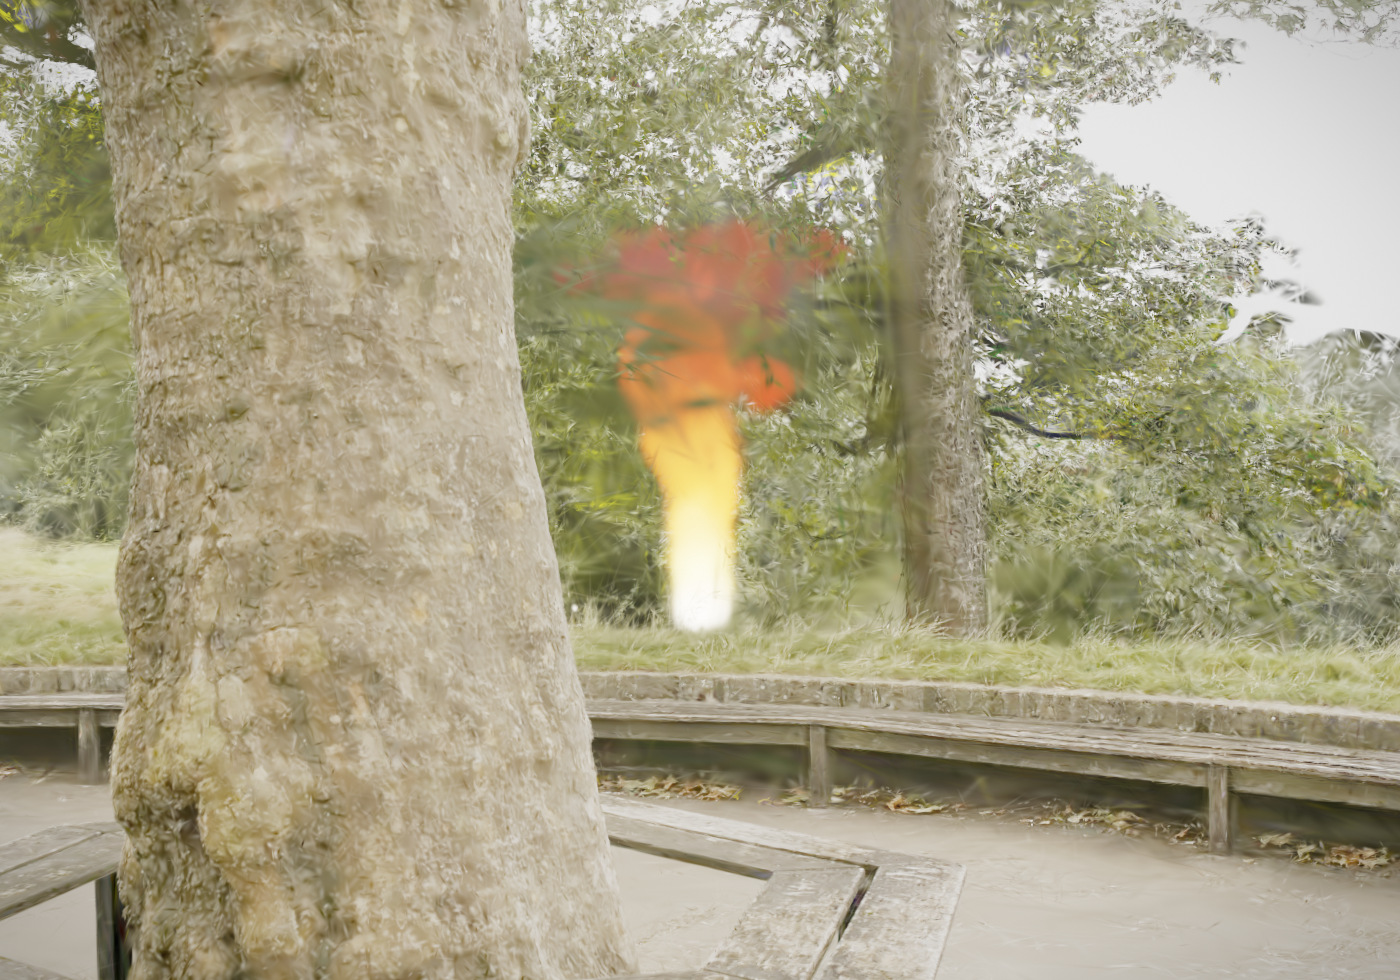
\includegraphics[height=2.72cm]{treehill_ours}\hfill
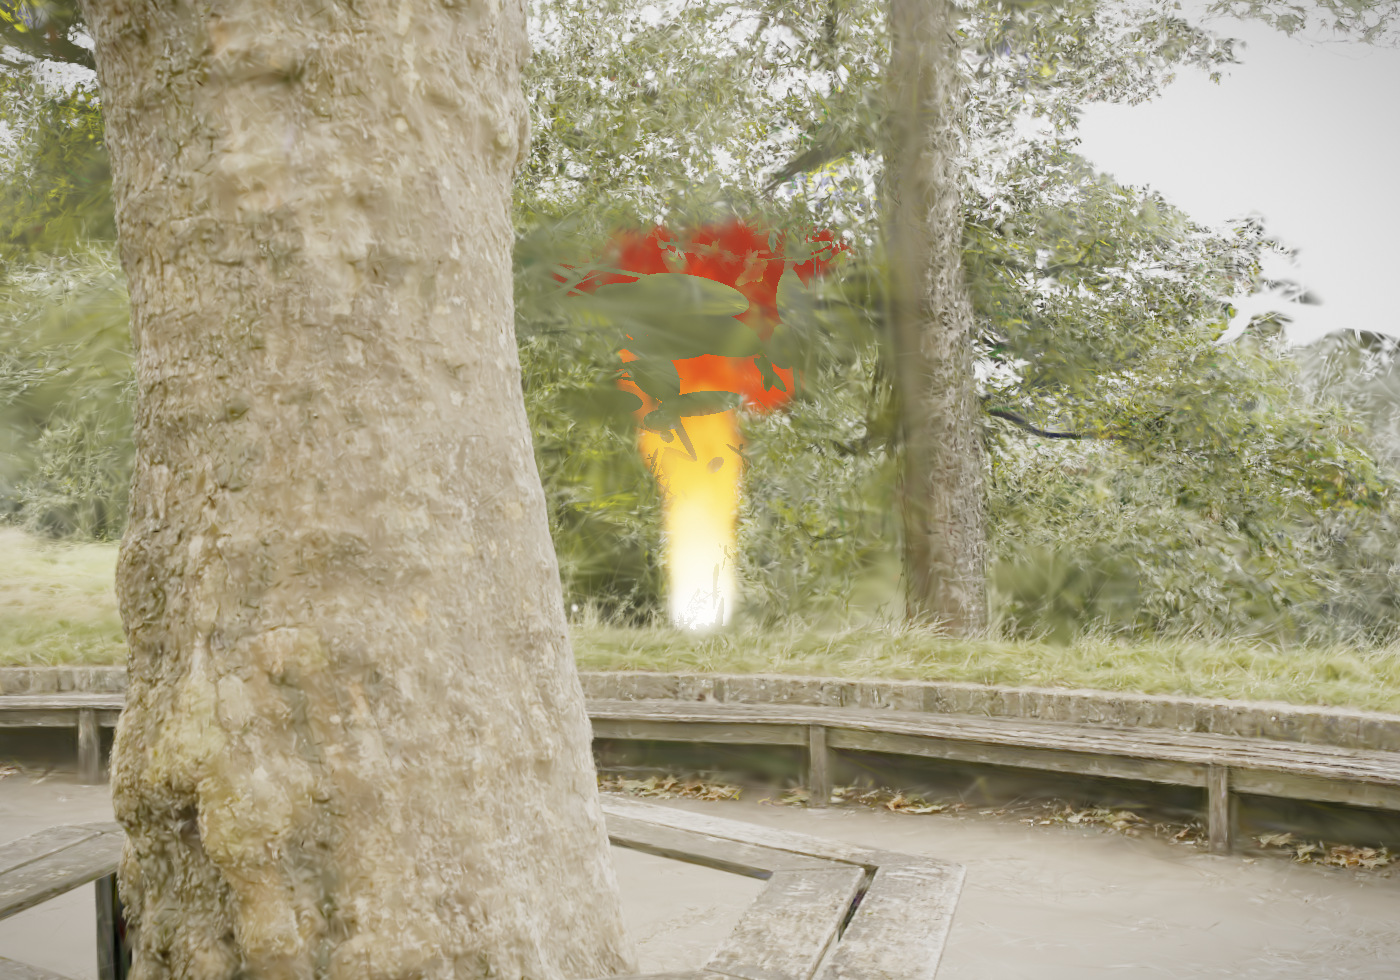
\includegraphics[height=2.72cm]{treehill_depth}\hfill
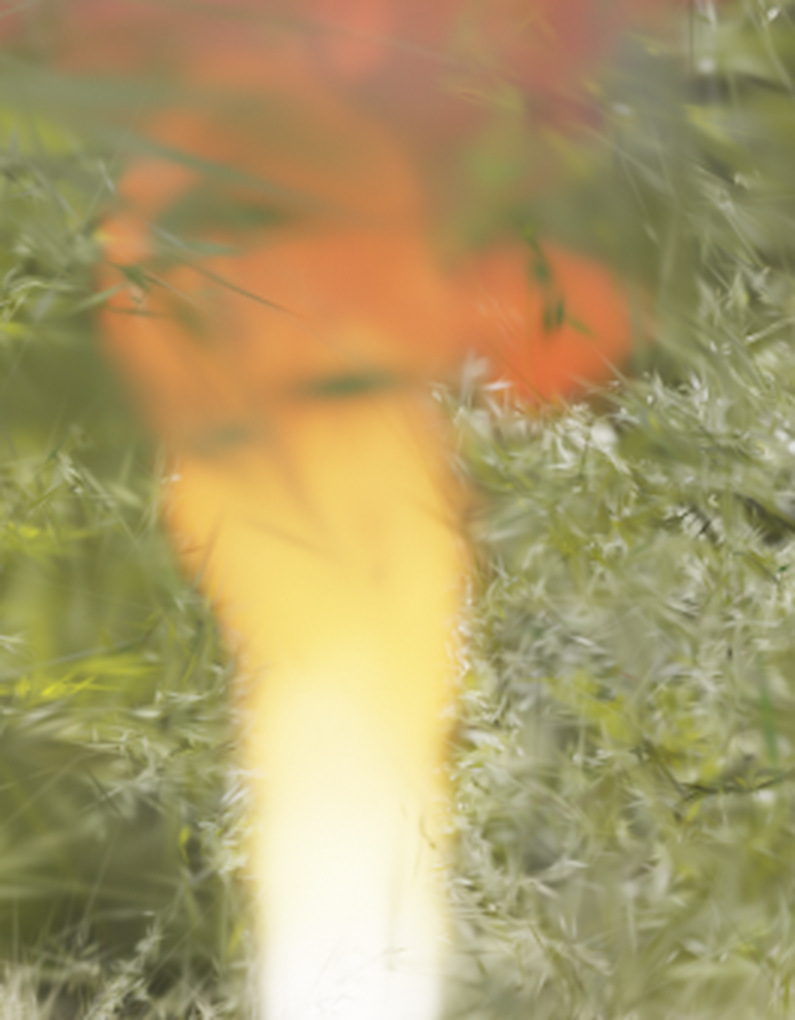
\includegraphics[height=2.72cm]{treehill_crop_ours}\hfill
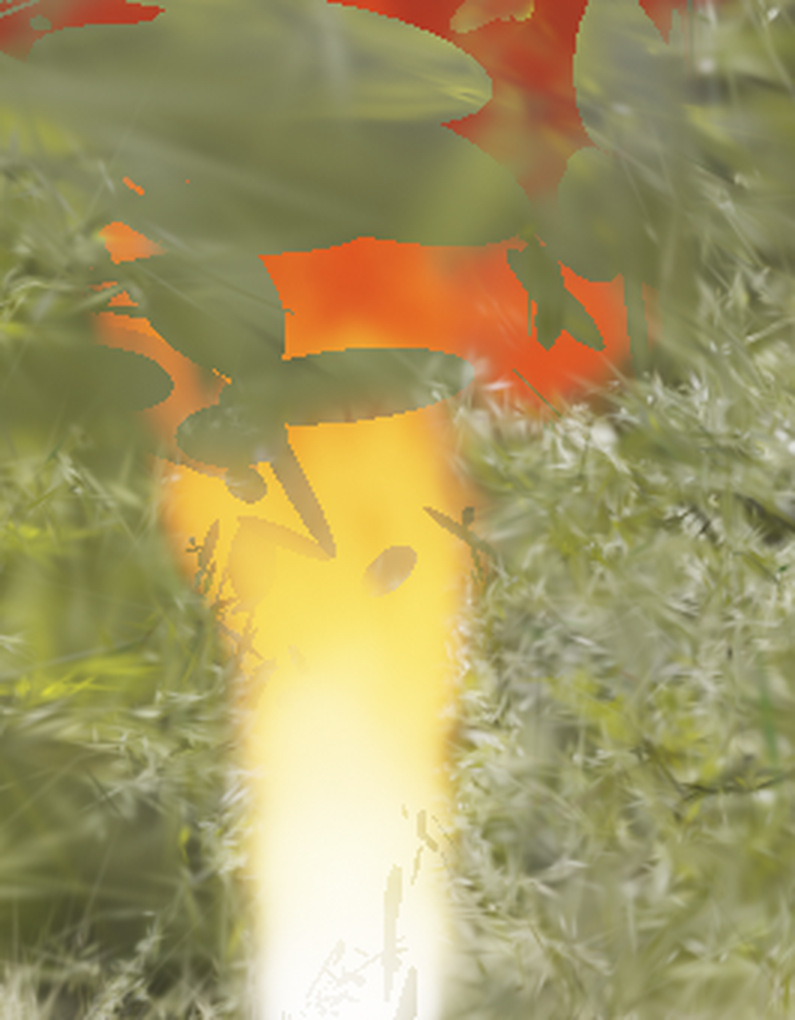
\includegraphics[height=2.72cm]{treehill_crop_depth}\hfill
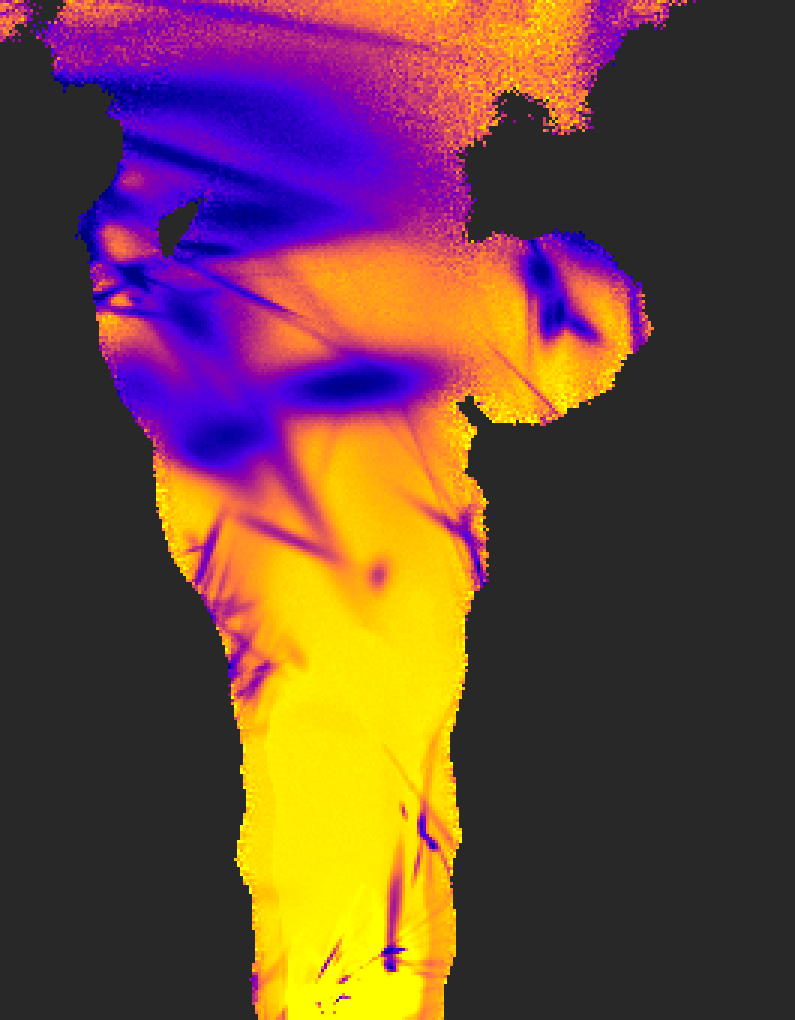
\includegraphics[height=2.72cm]{treehill_t_ours}\hfill
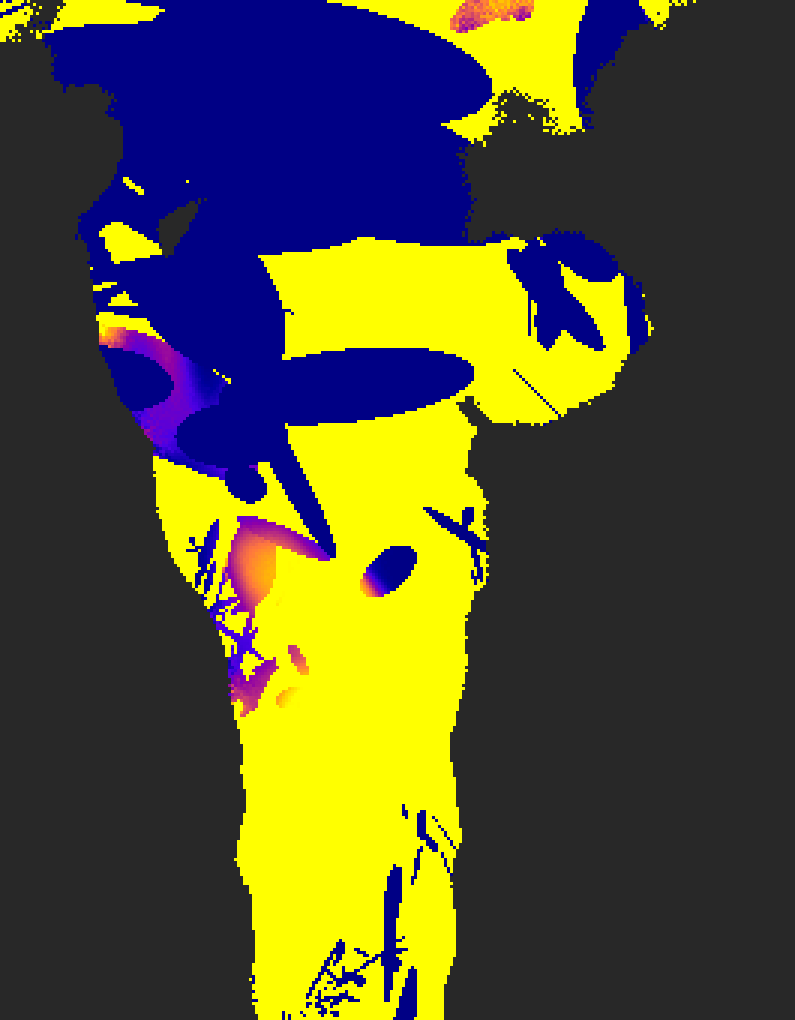
\includegraphics[height=2.72cm]{treehill_t_depth}
\caption{A semi-transparent occluder: \emph{treehill} at training camera \_DSC8979, selected by search over all eight Mip-NeRF 360 scenes on the fraction of silhouette with transmittance in $(0.05,0.95)$. Left to right: ours; depth-aware baseline at $\alpha=0.22$, the threshold matching our fire energy; $3\times$ crops of each; measured per-pixel transmittance of each. Simulation state is bit-identical in every panel. Over the 50\,355-pixel silhouette our transmittance histogram is continuous (mean 0.616, 88.1\% strictly partial). The energy-matched baseline is two spikes: 51.5\% fully open, 39.4\% fully blocked, 9.1\% partial.}
\label{fig:treehill}
\end{figure*}

\paragraph{Semi-transparent occluder.} On \emph{treehill} (2\,074\,009 Gaussians) a flame sits behind a clipped hedge, represented as a lace of low-opacity Gaussians (Figure~\ref{fig:treehill}). Transmittance is read from the renderer on its linear path by differencing two emissive gains, which cancels the scene term exactly; the unoccluded reference returns $T=1.0000$ over the whole silhouette. Our composition transmits partially at 88.1\% of pixels. The depth-aware baseline is bimodal at every threshold, with 0.6--9.3\% partial. Its energy can be matched, near $\alpha=0.235$, and its structure cannot: at the matched threshold 92.0\% of silhouette pixels differ from ours by at least 3/255. Excluding clipped pixels strengthens the result (96.6\% against 6.0--10.6\%).

The two captures together are the finding. Per-primitive interleaving and a per-pixel $z$-test agree on binary occluders and separate on semi-transparent ones, as the architecture predicts. The measurement rests on one capture and one viewpoint. We have not measured how the separation degrades as a reconstruction is thinned toward an interactive budget; the opacity floor that preserves the veil is 0.005, and raising it to 0.20 cuts the partial fraction from 93.8\% to 55.0\% on the offline instrument.

\subsection{The combustion loop}
\begin{figure*}
\centering
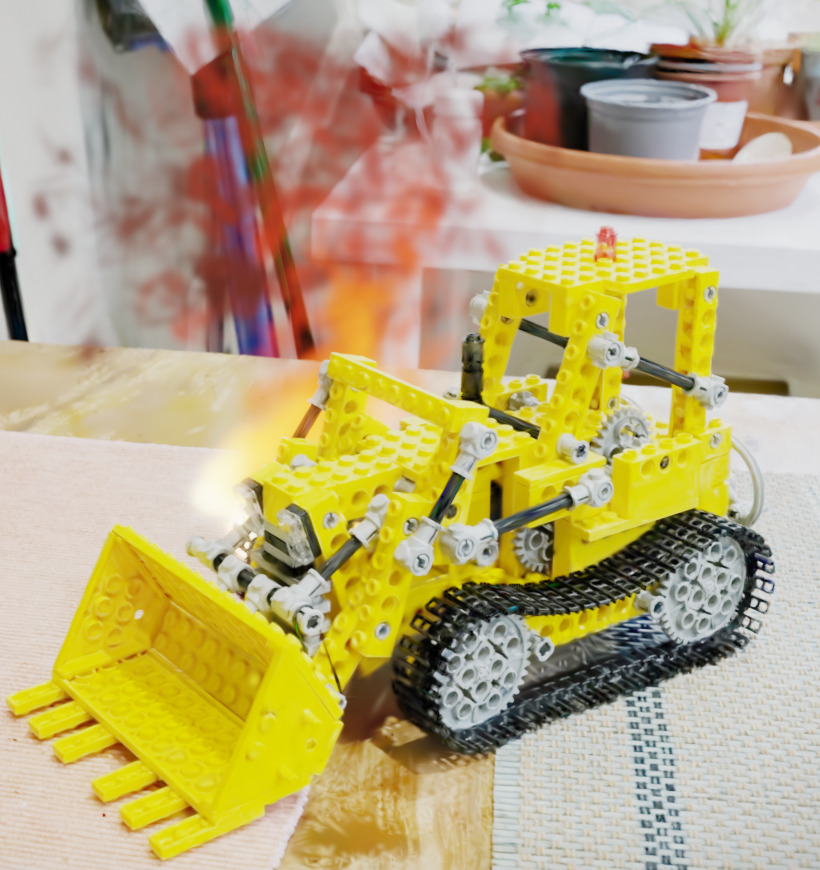
\includegraphics[width=.245\textwidth]{kburn_a}\hfill
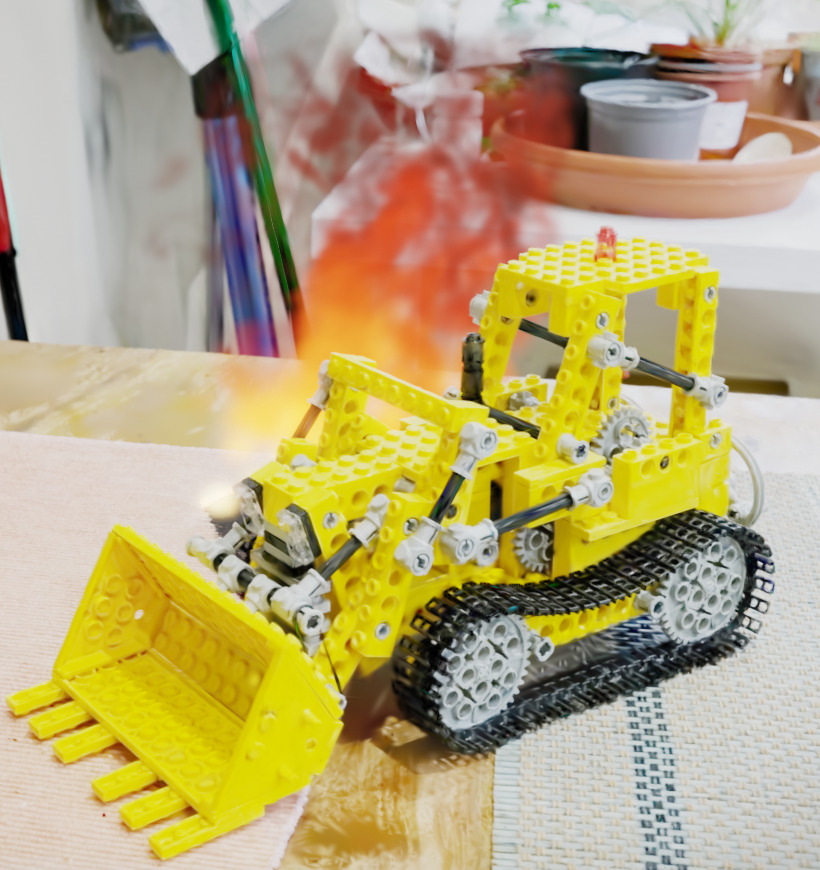
\includegraphics[width=.245\textwidth]{kburn_b}\hfill
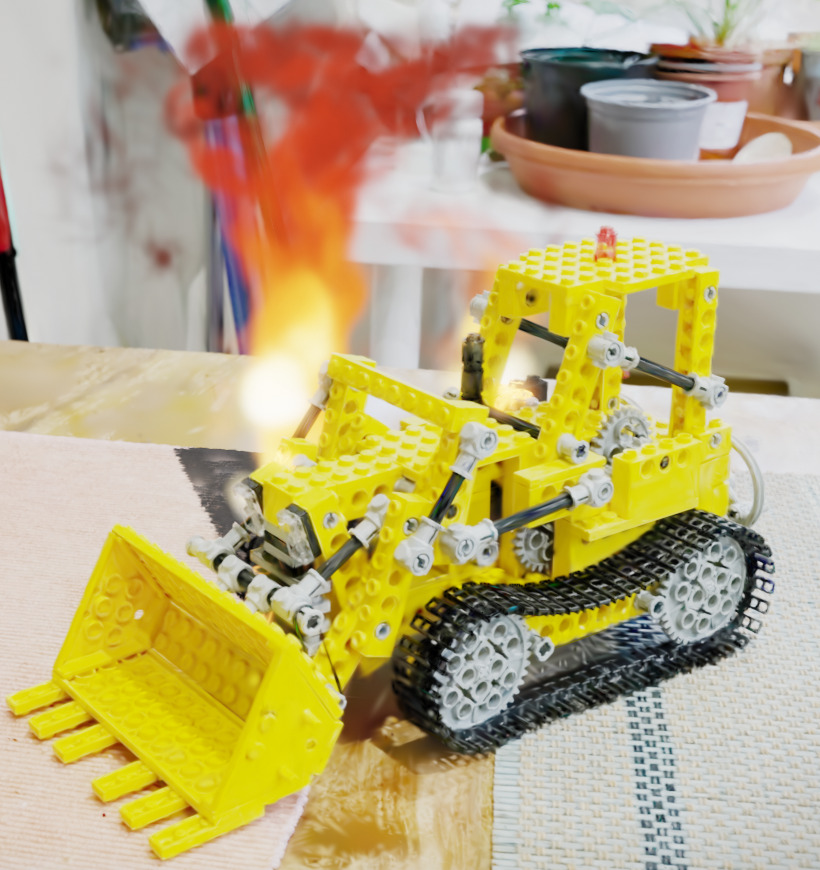
\includegraphics[width=.245\textwidth]{kburn_c}\hfill
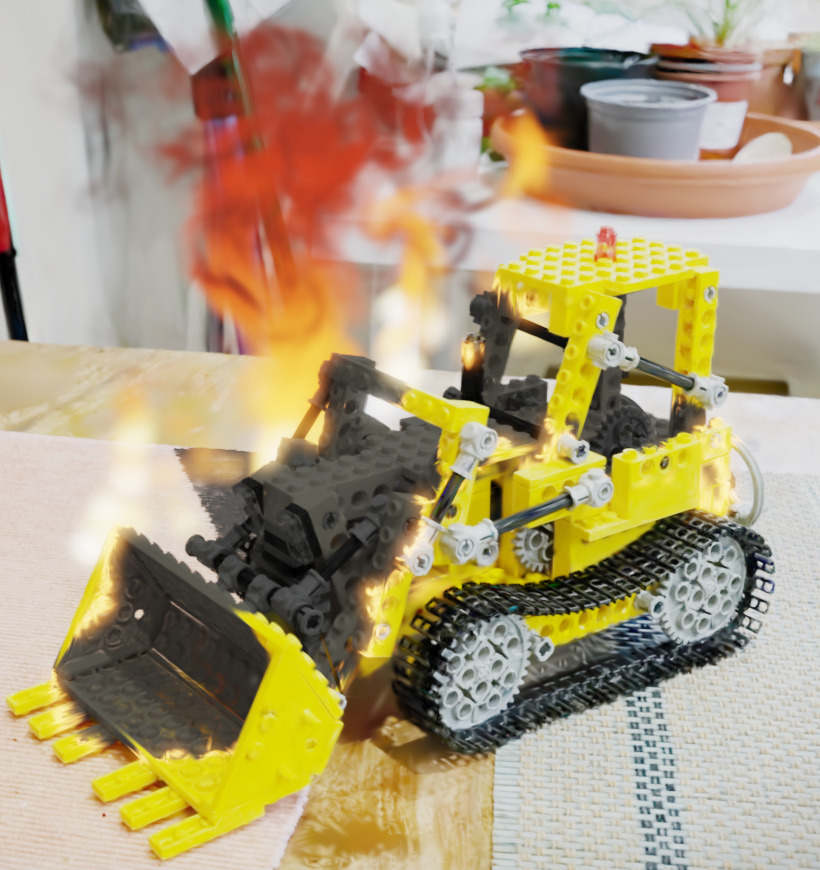
\includegraphics[width=.245\textwidth]{kburn_d}
\caption{The combustion loop on a public benchmark, with nothing ignited by hand. Fuel is a box around the loader (75\,443 of 729\,826 splats) and a thin strip of tabletop the flame stands in. Left to right: $t=11.95$\,s, the strip burns and the machine has received exactly zero heat; $t=24.40$\,s, the first 29 machine splats ignite; $t=99.83$\,s, 12.45\% of the machine lit; $t=249.73$\,s, 64.63\% lit and 41\,192 splats charred, with the run halted while still burning. Char is written into each splat's own albedo: over the 57\,252 charred pixels saturation falls 0.909 to 0.202 while surface relief survives.}
\label{fig:kburn}
\end{figure*}

Figure~\ref{fig:kburn} runs the loop on \emph{kitchen}. The flame stands 0.59 world units from the machine against a 0.14 heating radius, so it cannot reach it directly. The front crosses the fuelled table strip instead. The machine's splats read exactly zero heat through $t=11.95$\,s, heat first registers at $t=13.94$\,s, and ignition follows at $t=24.40$\,s. That delay is emergent: the system has no delay parameter, and a re-run reproduces the trace exactly. Containment held at all 56 checkpoints. The composited loop also closes on a 380k capture; the supplemental reports that run.

On a synthetic scene (45.8k splats) the loop runs in real time, with render 4.6 against 3.9\,ms quiescent at a $\sim\!190$-splat fire line. On captures it does not. A $1/60$\,s substep costs 99\,ms on the 380k capture and 146\,ms on \emph{kitchen} at comparable fire lines, and the whole \emph{kitchen} run averages 179\,ms over 15\,044 substeps: six to eleven times slower than real time. The frontier cap bounds how many burning splats are processed but not what each one costs, since the neighbourhood query scales with local splat density. On a capture, then, composition is limited by rasterization alone, while combustion is an offline effect. Making it interactive needs a coarser burn representation or a GPU frontier.

\subsection{Scene lighting and deflection}
\begin{figure}
\centering
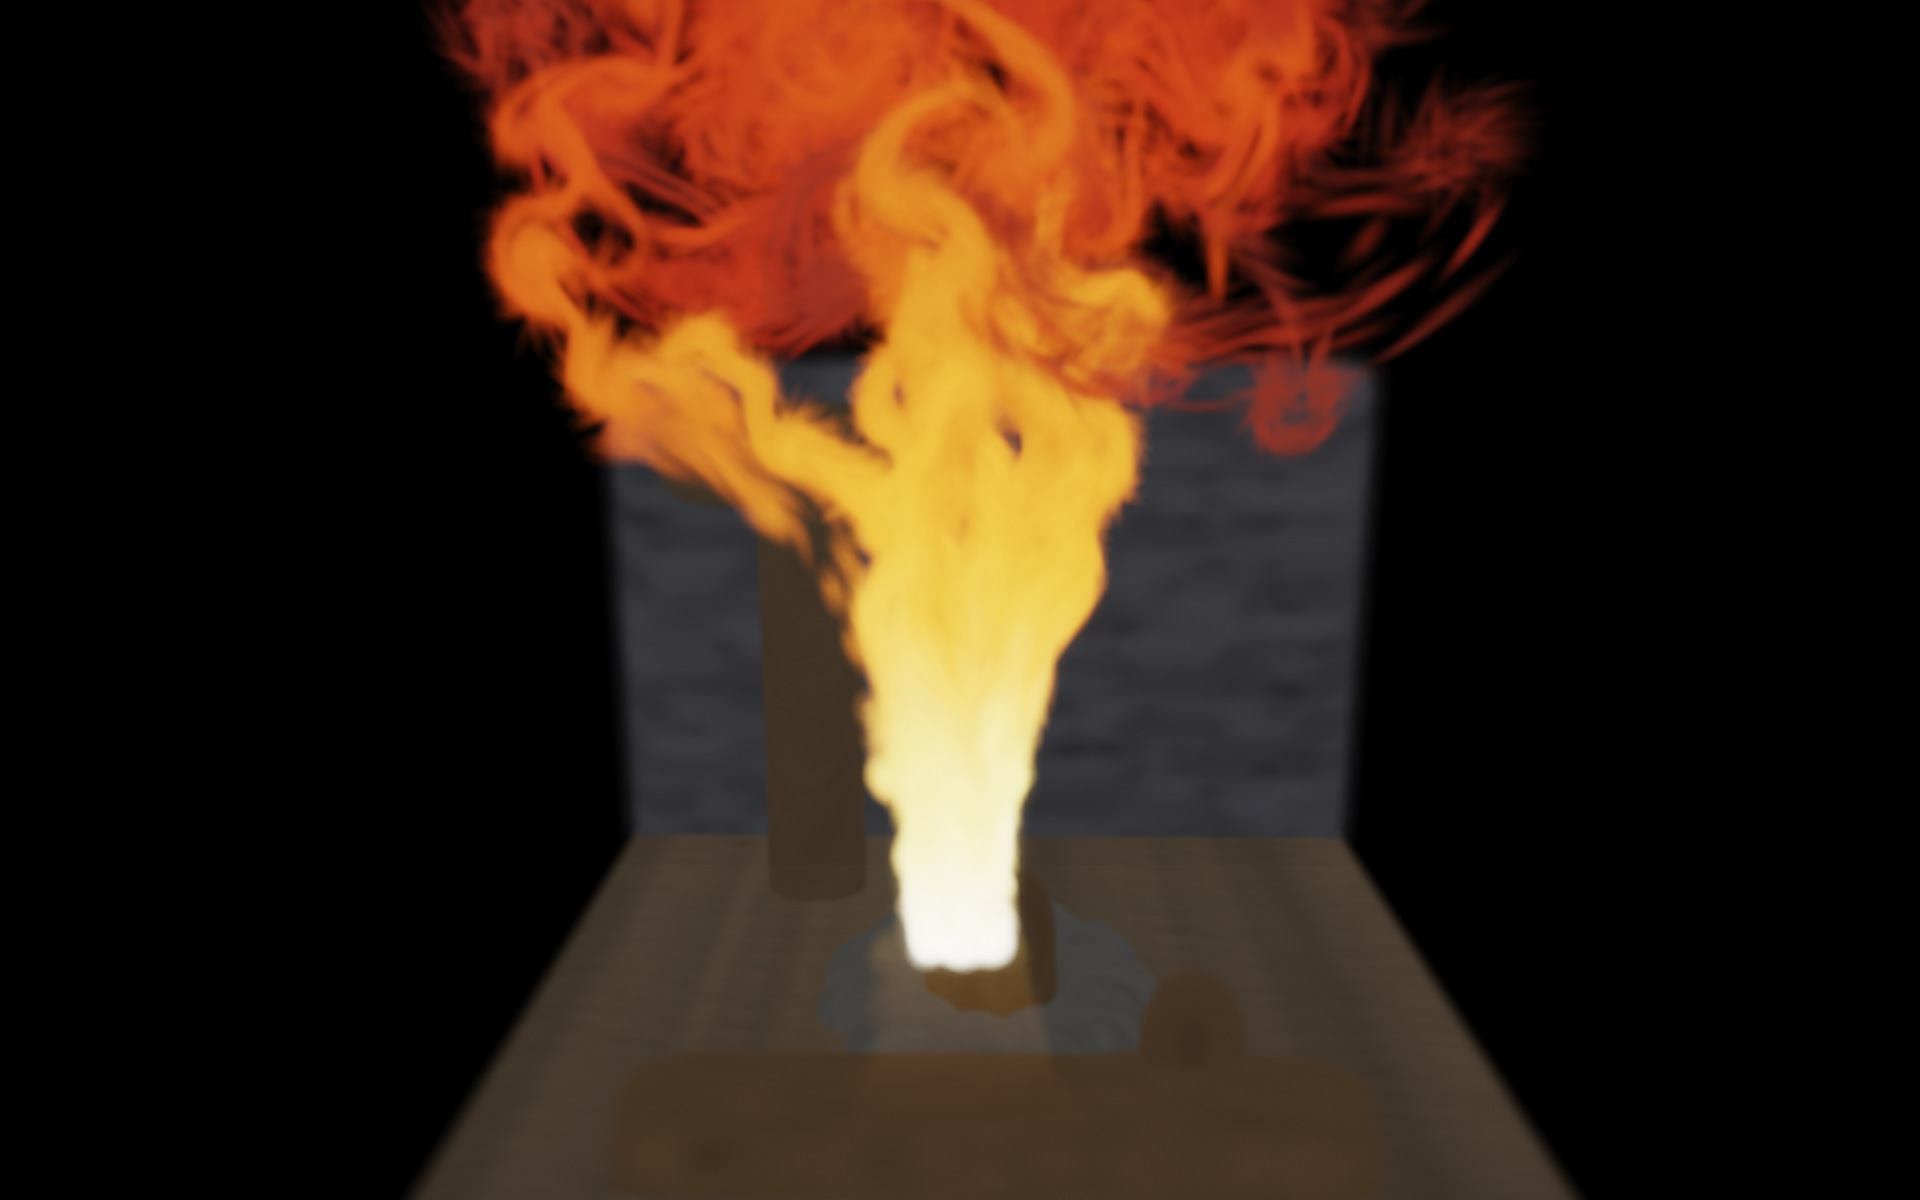
\includegraphics[width=.492\linewidth]{light_off}\hfill
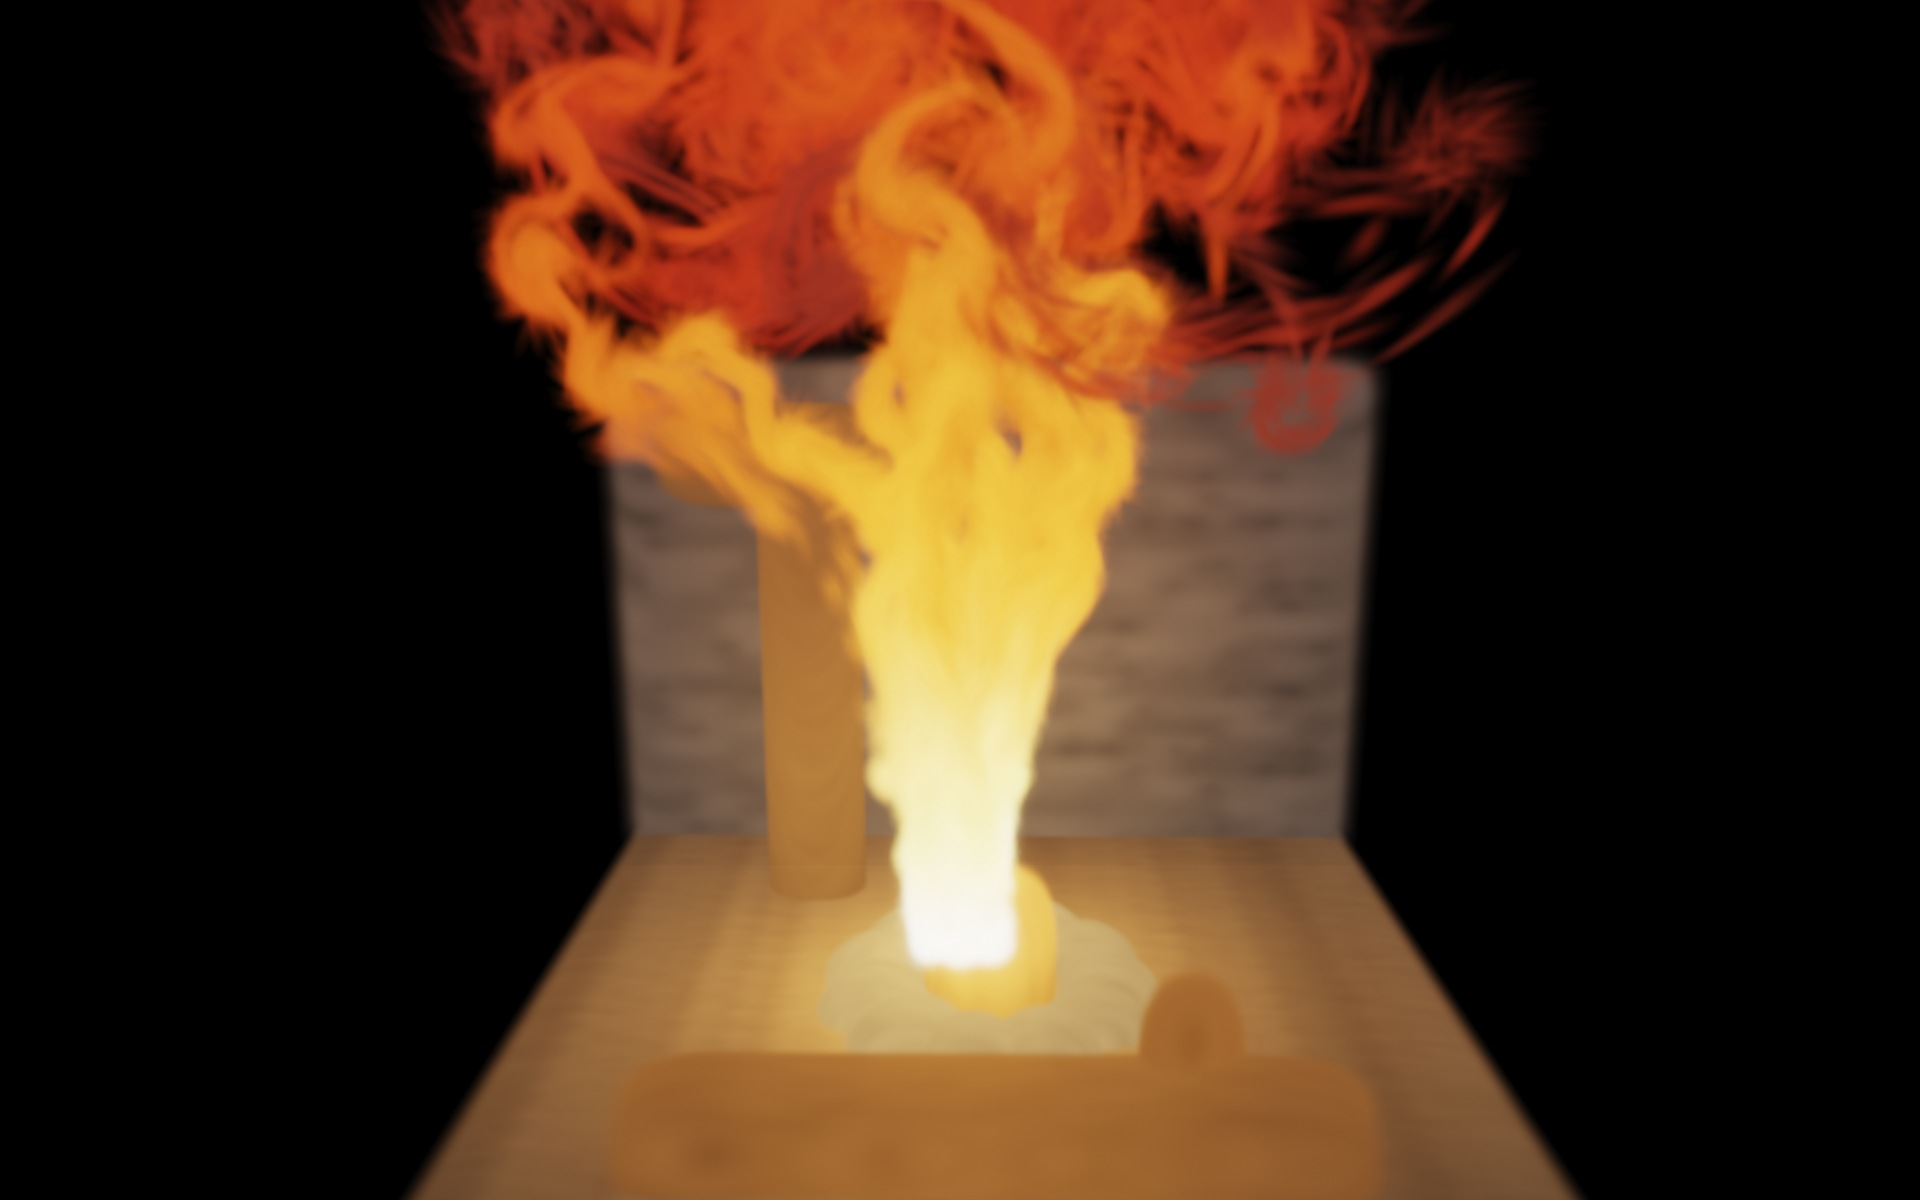
\includegraphics[width=.492\linewidth]{light_on}
\caption{World-space fire light (Eq.~\ref{eq:light}) on the synthetic scene at reduced scene brightness; identical state and camera, Hero preset. \emph{Left:} off. \emph{Right:} on; floor, wall, post and log pick up the flame's colour, and surfaces facing it brighten through the splat-axis normal.}
\label{fig:light}
\end{figure}

\paragraph{Light.} Figure~\ref{fig:light} shows Eq.~\ref{eq:light} on the 45\,808-splat synthetic scene. On the RTX 5070 Ti the frame stays at 11\,ms with the light on or off (10.97 and 10.80\,ms over 40 frames, a difference within measurement noise), and mean image value rises from 26.4 to 34.4. Replay hashes are identical to the build without it. Its cost scales with splats drawn, and we have not yet timed it at 729\,826 splats, so the capture rates in \S\ref{sec:cost} exclude it, while the scene rows of Table~\ref{tab:hw} include it. The teaser and Figures~\ref{fig:kitchen}--\ref{fig:kburn} predate this term and are rendered without it.

\begin{figure}
\centering
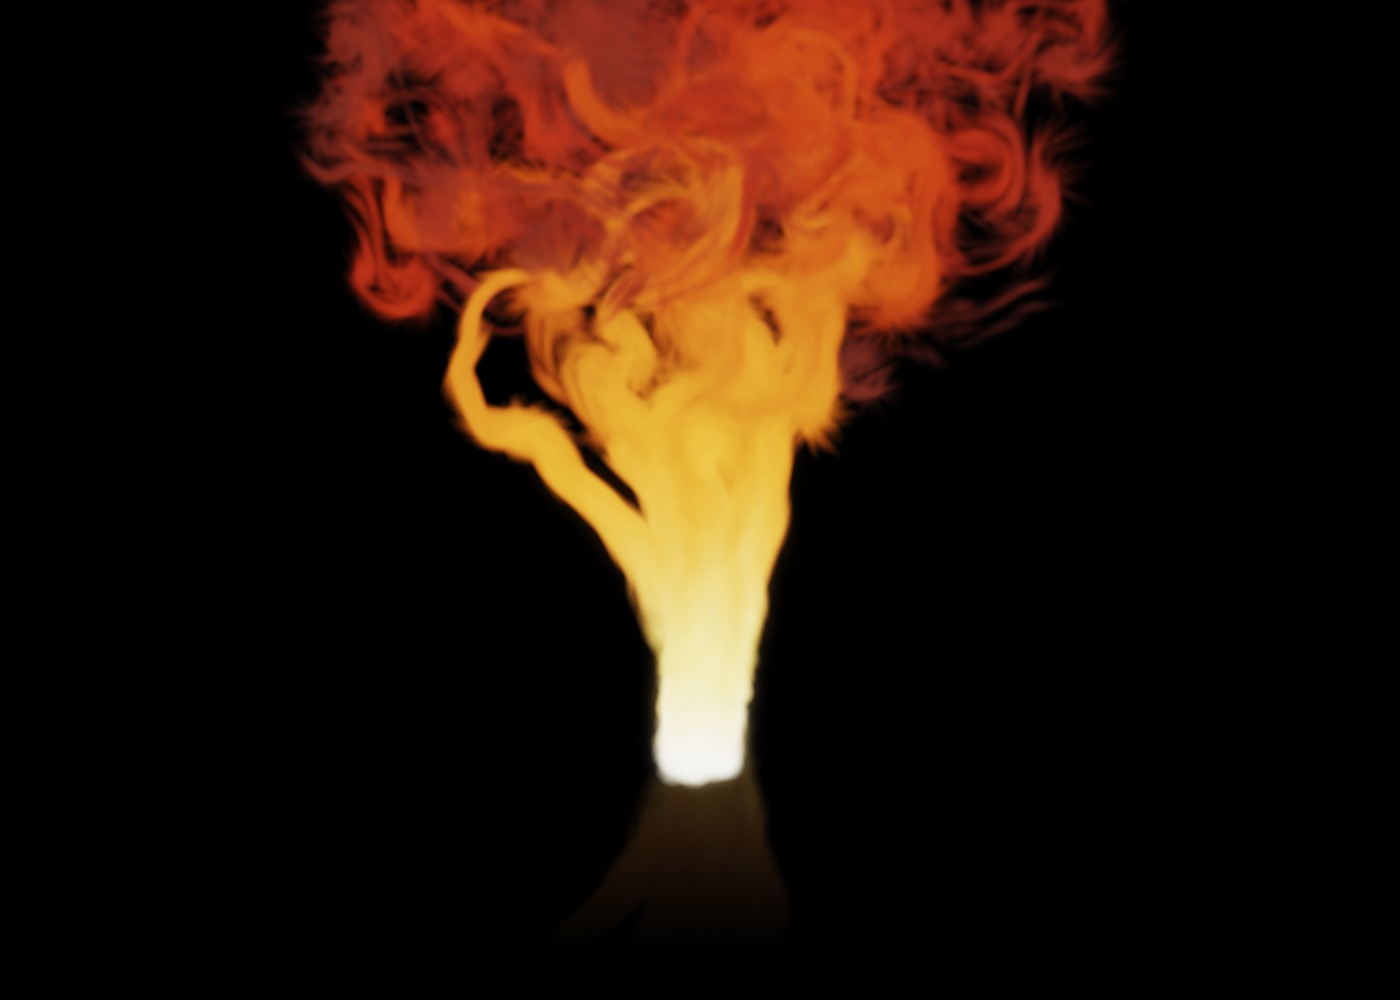
\includegraphics[width=.492\linewidth]{deflect_off}\hfill
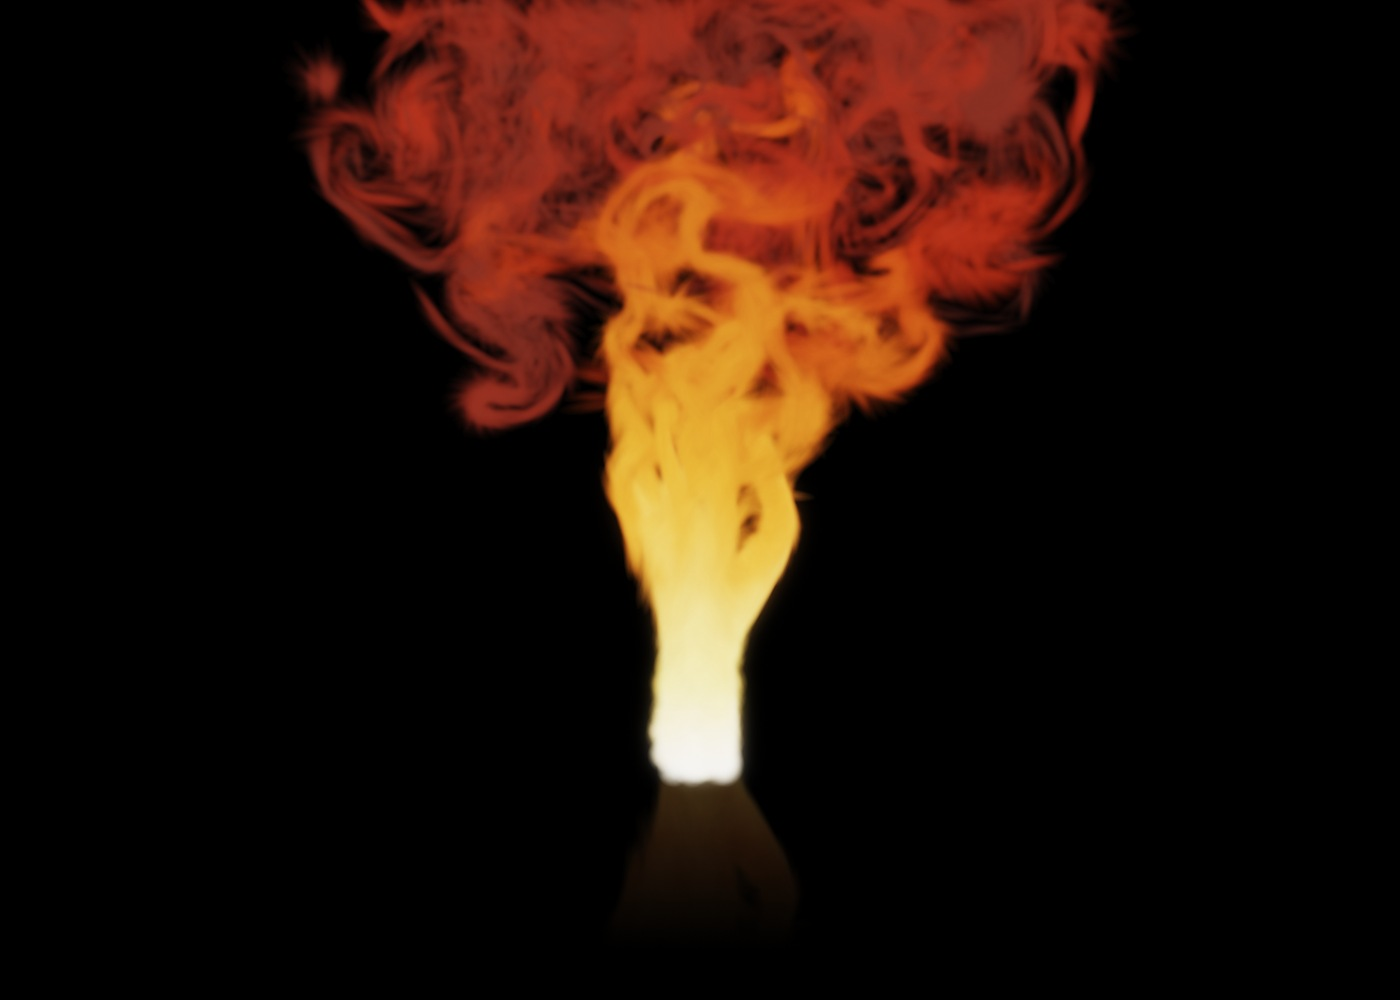
\includegraphics[width=.492\linewidth]{deflect_on}
\caption{Deflection around a sphere of radius 0.24 on the plume axis at $y=1$; same seed, Hero preset. \emph{Left:} the flame passes through it. \emph{Right:} the boundary terms of \S\ref{sec:deflect} split the plume, and the wake rolls up.}
\label{fig:deflect}
\end{figure}

\paragraph{Deflection.} We place a sphere on the plume axis, world-fixed slices, interactive preset, and compare the path off and on over eight seeds, sampling hot particles after 360 steps (Figure~\ref{fig:deflect}). Hot particles inside the sphere fall from 4.08\% to 0.00\%. Particles on the axis at sphere height fall from 81\% to 55\%, and the plume above it widens from 0.144 to 0.200. With twelve spheres in the path the simulation step rises from 4.54 to 4.93\,ms. Automatic proxies build on the synthetic scene, 48 spheres at the cap, with stable runs. We have not yet exercised them on a capture, so the \emph{kitchen} plume in Figure~\ref{fig:kitchen} remains undeflected, and proxies are coarser than thin geometry. A sphere proxy cannot follow the loader's arms.

\subsection{Grid-free solver and treecode}
\label{sec:treecode}
\begin{figure}
\centering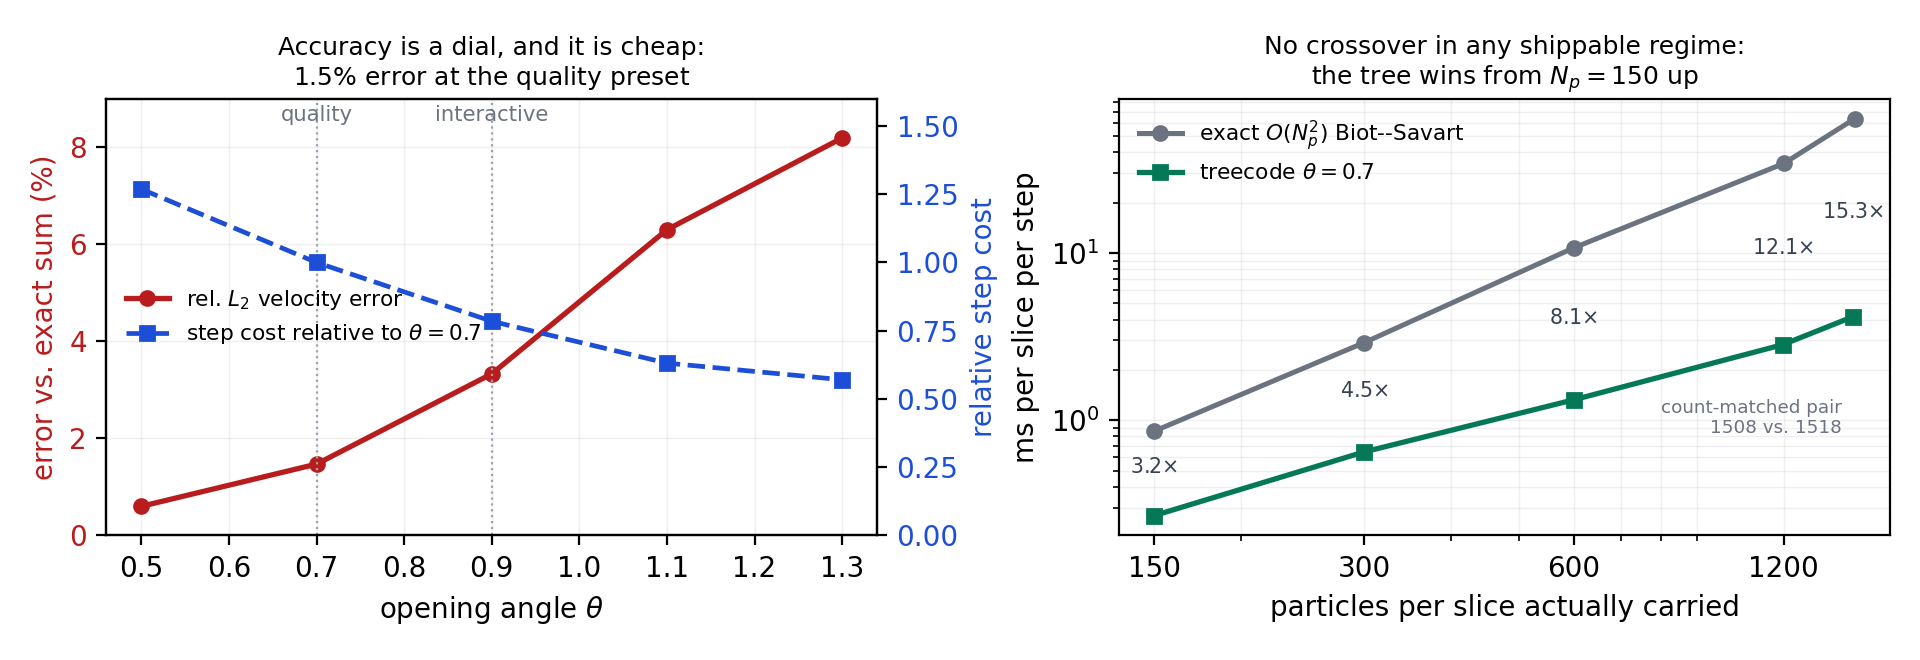
\includegraphics[width=\linewidth]{treecode}
\caption{The treecode against the exact sum. \emph{Left:} relative $L_2$ velocity error against opening angle. \emph{Right:} per-slice cost; the treecode is faster at every count we can ship, from $3.2\times$ at $N_p=150$ to $15.3\times$ at $\sim\!1.5$k.}
\label{fig:treecode}
\end{figure}

Figure~\ref{fig:treecode} prices the treecode. Relative $L_2$ velocity error is 0.6, 1.5, 3.3 and 6.3\% at $\theta=0.5,0.7,0.9,1.1$, and there is no crossover against the exact sum in any regime we can ship. Against the retained vortex-in-cell baseline at matched counts, the grid-free step costs $2.3\times$ more at the quality preset (29.8 against 12.9\,ms) and $1.3\times$ more at the interactive preset. The return is measured in the next section.

Perceived detail is bounded by the particle budget. The on-screen radius never enters the solver, and shrinking it sharpens the image only until blobs stop tiling, at which point the overlap condition $h\lesssim\sigz$ fails visibly.

\subsection{The layered approximation}
\label{sec:layered}
\begin{figure}
\centering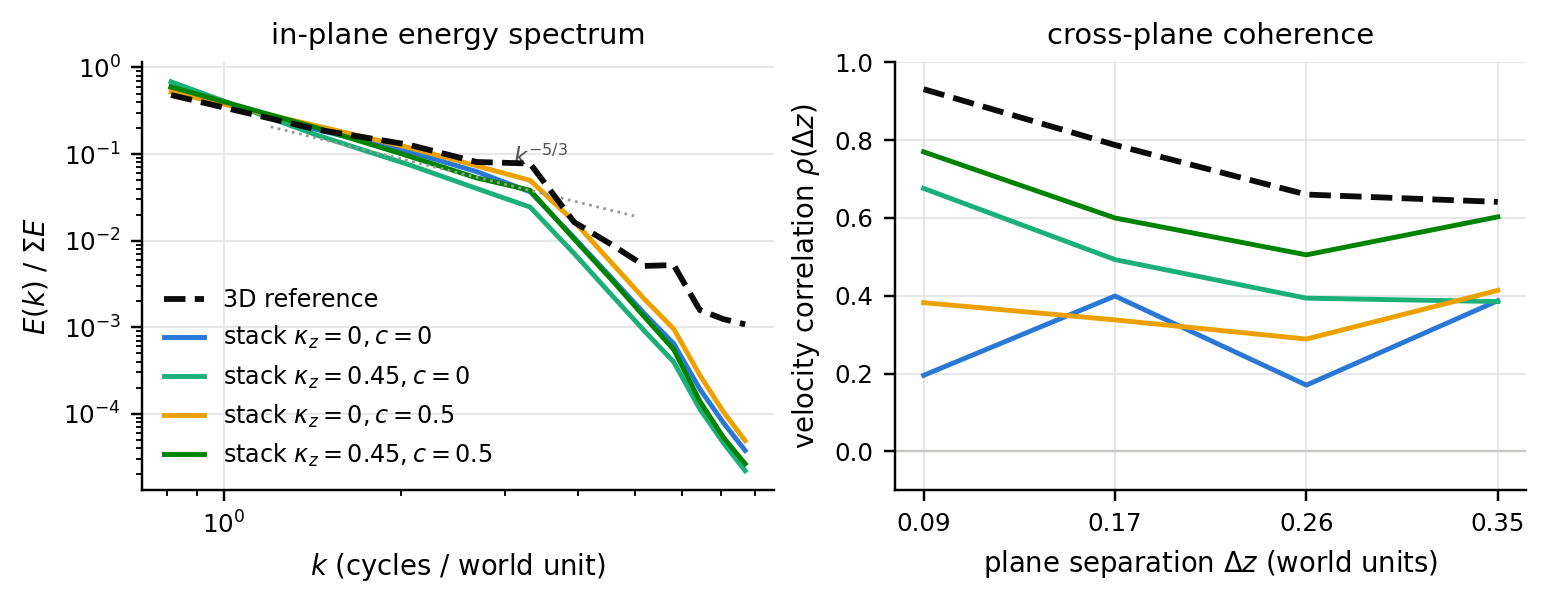
\includegraphics[width=\linewidth]{spectra}
\caption{Against a matched true-3D Boussinesq reference (dashed). \emph{Left:} normalized in-plane spectra. \emph{Right:} cross-plane velocity correlation. Curves show one seed; values in the text are four-seed means.}
\label{fig:spectra}
\end{figure}

We compare the stack with two 3D controls under one protocol (Figure~\ref{fig:spectra}): an external $32\times48\times32$ Boussinesq Euler solve, and a true 3D Gaussian vortex-particle solver built inside the prototype, sharing kernel family, $\sigz$, $\theta$, budget, source terms and renderer. All figures are means over seeds $\{7,11,17,23\}$.

\paragraph{In-plane spectra.} The reference holds 48\% of its energy in the largest-scale bin and $\sim\!30\%$ in the mid-band. Across configurations the grid-free stack holds 50--67\% and 15--27\%, at log-spectral distance 0.39--0.68. The vortex-in-cell stack, through the identical protocol, concentrates 83--92\% in the largest bin with 2--5\% mid-band, at 0.78--0.87. This is the measured return on grid freedom. A $64\times96$ grid recovers shape at higher cost than the grid-free solver at $9\times1300$, and on the band carrying 97.7\% of reference energy it scores 0.24--0.34 against 0.13--0.16.

\paragraph{Coherence.} Adjacent reference planes correlate at $\rho\approx0.93$ and the matched 3D control at 0.80. The uncoupled stack sits at 0.18, and coarse coupling raises it to 0.29. The exchange of Eq.~\ref{eq:pse} raises it to 0.62 alone and 0.76 combined with $c$, at a spectral price: distance moves 0.53 to 0.68 alone and 0.39 to 0.54 with $c$. A blur null shows the coherence is the operator's: in-plane diffusion buys $+0.04$ in $\rho$ for $+3.3$ in distance, against $+0.44$ for $+0.15$.

\paragraph{Stretching.} Under the grid-free pair the stack-to-3D distance is 0.28--0.40, and switching vortex stretching off inside the 3D solver moves its spectrum by only 0.06, about 20\% of that gap. The rest is the loss of three-component transport. The 3D solver at matched budget costs $2.8\times$ the stack's step, so layering is not what makes the system real-time. It buys resolution allocation: in-plane detail is cheap and depth is charged per slice. At equal wall-clock cost the 3D solver reaches a better spectrum but only 1.9k renderable Gaussians, too few to tile a flame. A system free to simulate on one element set and render on another would prefer it. Ours is not, by construction.

\subsection{Beyond the browser}
The solver is not tied to the prototype. Compiled as dependency-free C++17 and run headless, it burns a drone reconstruction of a village inside NVIDIA Omniverse (Isaac Sim 6.0), where reconstruction, flame, smoke and char are one OpenUSD 26.03 \texttt{ParticleField3DGaussianSplat} primitive type, ray-traced in a single pass. The shot renders 1\,892\,830 static Gaussians plus the 736\,360 of a farmhouse; 220\,706 splats burn at the peak and 400\,000 are charred by the last frame, 54\% of the building. This is an offline render, 15\,s at $1920\times1080$ with playback speed equal to simulation speed, and it shows that the primitive identity survives a change of renderer. We did not measure it against the rasterized path, and it carries no timing claim.

\subsection{Offline quality}
\label{sec:hero}
For stills and video we use a Hero preset: $9\times3000$ at $\theta=0.7$, on-screen radius 20 rather than 42, a raised emission rate, and lower emissive gain so the core keeps structure instead of clipping. The population rises to 26.2k Gaussians and mean image gradient from 0.37 to 0.43 against the quality preset (Figure~\ref{fig:hero}). It is the same solver and renderer with more elements, and it is not an interactive configuration.

\begin{figure}
\centering

\includegraphics[width=.492\linewidth]{fire_quality}\hfill
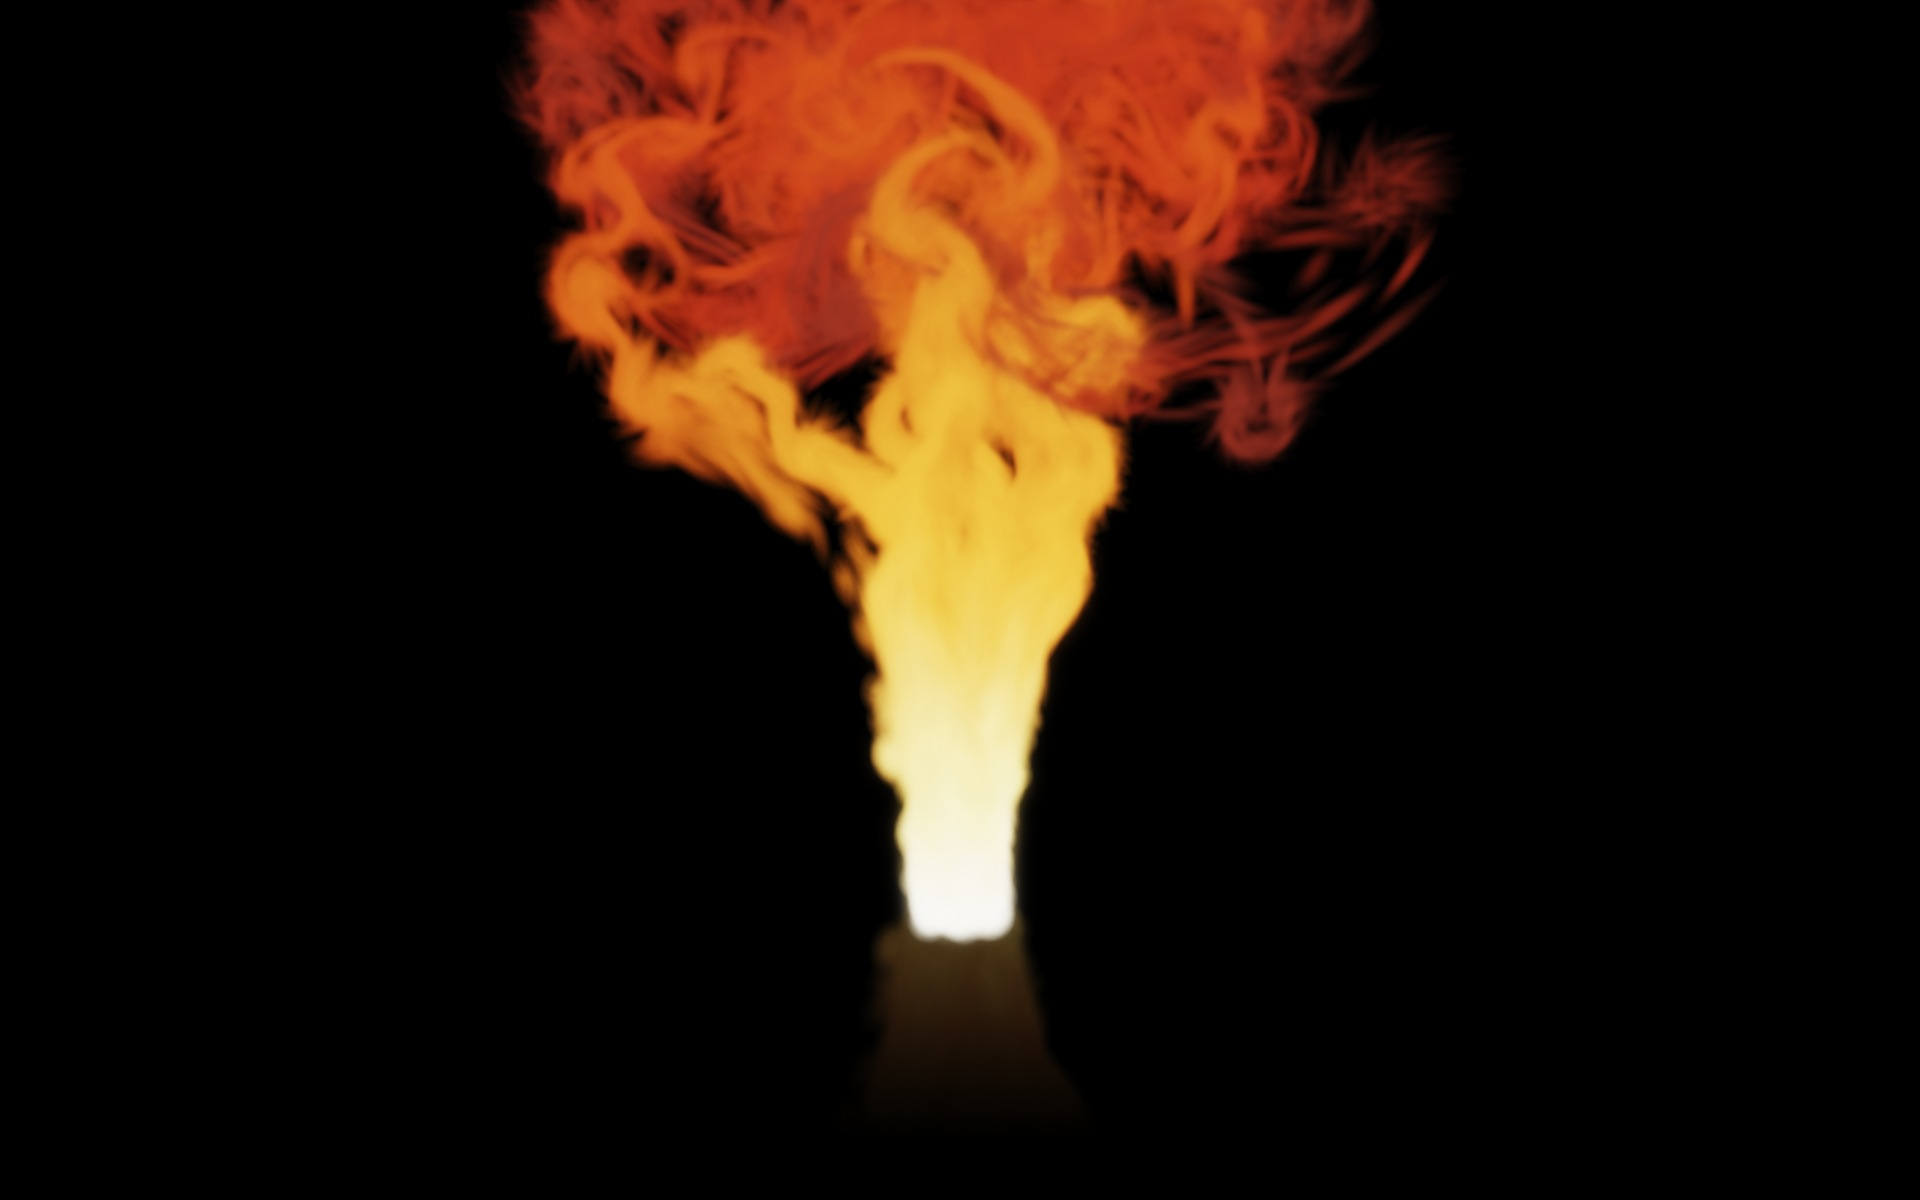
\includegraphics[width=.492\linewidth]{fire_hero}
\caption{\emph{Left:} quality preset. \emph{Right:} Hero preset, same seed and step count. Spending elements resolves filaments the interactive budgets cannot tile.}
\label{fig:hero}
\end{figure}

\subsection{Perceptual evidence}
Our central trade, physical fidelity for interactivity in a medium where the eye is forgiving, is an empirical claim about viewers, and at the time of writing it is untested. The instrument is released and pre-registered: a two-alternative forced choice over five ablations, 18 trials, 4\,s looping clips with deterministic pairs, analysed by pooled two-sided exact binomial tests with Wilson intervals and a per-participant direction count, with no outlier rejection and a target of $N\geq12$. Composition is excluded by design, since its claim is structural and is settled by measured transmittance (\S\ref{sec:occlusion}).

\section{Limitations and Future Work}
\paragraph{Layered physics.} A slice stack cannot reproduce 3D turbulence statistics. Figure~\ref{fig:spectra} is the standing target for any coupling design, and Eq.~\ref{eq:pse} recovers coherence at a measured smoothing price without supplying stretching amplification.

\paragraph{Illumination.} Eq.~\ref{eq:light} is direct diffuse light from six clusters. It has no shadows, no specular term and no volumetric scattering, and it treats baked radiance as albedo. FieryGS adds a specular term and integrates more source voxels at far greater cost. Cast shadows and smoke self-shadowing are future work.

\paragraph{Deflection.} Sphere proxies are coarse, proxies are static so burnt geometry does not vacate them, and the wall term is a surrogate for a boundary layer rather than a no-slip solution. The ideal generalization replaces Eq.~\ref{eq:doublet} with boundary vortex Gaussians whose strengths come from a panel method.

\paragraph{View dependence.} View-aligned slices make the fire's world-space geometry a function of the camera, the sharpest tension in the GS-native framing: attributes are camera-independent while the lift is not, so stereo eyes see slightly different fires. The world-fixed mode removes this at the cost of edge-on collapse. Fast camera motion and flows along the view axis remain the weakest cases \cite{horvath2009}.

\paragraph{Scale.} What leaves the real-time budget in a large scene is rasterization, for which tile-binned GPU sorting and level of detail are the natural route. Optically thin fire suggests a radiance-conserving criterion distinct from photometric LOD \cite{kerbl2024}. Fuel assignment remains a hand-drawn box, and deciding what burns from a reconstruction alone is a segmentation problem we do not address.

\section{Conclusion}
Fire and smoke can live inside Gaussian-splatting scenes as the primitives those scenes are made of. Because vortex elements and splats are one population, a flame transmits partially through captured foliage where a depth test cannot, burns on the reconstruction's own primitives, lights it and is deflected by it, with no grid and no linear solve between solver and pixels. The fire alone is real-time on a desktop and interactive on integrated graphics; composition with a large capture and combustion on it are not yet, and each of those costs is measured here. We expect the same unification to extend to other optically thin Lagrangian phenomena such as sparks, spray and dust.

\bibliographystyle{ACM-Reference-Format}
\input{refs.bbl}
\end{document}
